%\chapter{Bayesian Neural Networks for Cancer Types Prediction}
%\chapter{Neuro-symbolic Representation Learning on Knowledge Graphs}
\chapter{Symbolic Decision Reasoning}\label{chapter:nsr}
\textit{``AI will create a suite of ML techniques that enables human users to understand, appropriately trust, and effectively manage the emerging generation of AI partner''}- David Gunning

\section{Chapter Overview}
%\section{Symbolic reasoning}
In the previous chapter, we deduced rule set to explain individual diagnostic decision to end users. However, how do we know that the feature in the antecedents are biologically significant, given that until now we haven not incorporated any domain knowledge in the model. In other words, we feed the model with training data and clinical outcome, which then learned a bunch of hyperparameters. We have seen our models can predict cancer types with high level of confidence. However, carcinogenesis is not only about predicting something with high accuracy, but also understanding true biological meaning. One of the first steps to improve an XAI system is to understand its weaknesses, while the weakness analysis on `black-box' models is not straightforward than models that are interpretable~\cite{bhatt2020explainable}. The better we understand what a model explains, e.g., why and how it works or fails in certain cases and which factors caused it to make a given prediction, the easier it becomes to improve it. An efficient ML model that is better at predicting, detecting, and processing patterns than human, may not be able to reason its decision~\cite{miller2018explanation}. 

\hspace*{3.5mm} As we already argued that in sensitive contexts where the impact of AI on human life is relevant, e.g., medical diagnoses, explainability is not only a desirable property, it will~\cite{futia2020integration} or already become a legal requirement with the EU GDPR. In addition to predictions and explanation from the model, reasoning capability is desirable such that a model can reason about entities and eventually answer queries posed by human operators in order to guide decision making processes. Until now two more questions evolved: i) why should a physicians, for example trust the provided diagnosis decision?, ii) will `black-box' methods contribute to advancement of science with only numbers, not insight? One motivation is that a lots of what we know about drugs, genes, protein, viruses, and their mechanism is spread across a huge number of scientific articles. From the perspective of `XAI' and `context understanding', research~\cite{oltramari2020neuro} has derived that a corollary that suggests `the explainability of AI algorithms is related to how context is processed computationally, based on the machine's perceptual capabilities and on the external knowledge resources that are available'. This emphasizes on the context understanding, which can only be attained with neuro-symbolic architectures that is capable of instructing machine perception~\cite{oltramari2020neuro} by introducing semantics into neural networks, i.e., knowledge graphs~(KGs)-based reasoning with DNN.

\hspace*{3.5mm} Subsequently, research initiatives also now gradually adopting Semantic Web~(SW) technologies~\cite{karim2018improving} such as KGs, knowledge bases~(KBs), and domain-specific ontologies as a means of building structured networks of interconnected knowledge~\cite{futia2020integration} about drugs, genes, and proteins that can help in diagnosing cancer. Those articles can be used as a large-scale knowledge source and be be of huge impactful in disseminating knowledge about mechanism of carcinogenics. For example research~\cite{POSTF} has exposed that some genes have both oncogenic and tumor-suppressor functionality called  proto-oncogenes with tumor-suppressor function~(POTSF). Most of the POTSF genes act as transcription factors or kinases and exhibit dual biological functions, e.g., that they both positively and negatively regulate transcription in cells. There are some specific cancer types, e.g., leukemia are over-represented by such POTSF genes, whereas some common cancer types like lung cancer are under-represented by them~\cite{POSTF}. To answer these questions, we cover how the symbolic reasoning~(SR) help inferred and validate domain knowledge about top-k biomarkers we identified in the previous chapters. 
%Besides, we perform knowledge matching to validate the diagnostic decision. 
We hypothesize\footnote{\textbf{H5}: Based on a set of axioms and explicit facts, ontological reasoning technique can characterize diagnosis decision by inferring implicit but previously unknown facts} that ontological reasoning can infer new knowledge from existing knowledge and axioms. In other words, based on a set of axioms and explicit facts, a semantic reasoner will able to derive implicit but previously unknown facts from a KB. 

\section{Introduction}
Humans usually communicate with signs and symbols, what we desire from machines too. Combinations of symbols that express their interrelations is refereed as reasoning. When humans combine a bunch of signs together to express something meaningful, we call it symbolic manipulation. However, in many scientific process, `proof' simply doesn't exist, i.e., there can only be facts and evidence that can lead us to certain conclusions. In such a case, either deductive or inductive reasoning is used to reach a specific logical and true conclusion or to express complex thought based on symbolic relations.%, e.g., the old Roman chestnut: \texttt{`All men are mortal; Caius is a man; therefore Caius is mortal'}.
A complementary approach is symbolic AI, where symbols are elements of a \textit{`lingua franca'} between humans and deep learning~(DL)~\cite{janssens2007dynamic}. Semantic AI fuses symbolic and statistical AI, where methods from machine learning, knowledge modeling, and SW technologies are combined, making semantic reasoning and neural networks are the future to realize and build such an XAI system. KGs and their underlying SW technologies are the modern implementation of symbolic AI, while being less flexible and robust to noise compared to DL models, KGs are natively developed to be explainable. 

\hspace*{3.5mm} Therefore, research considers introducing semantics into DL through ontological reasoning a new era towards XAI, where a DL model reads input data, generates the predictions, observe the results, use the existing knowledge from the KB as a semantic reasoner, and produces new knowledge to provide more human-interpretable answers and explanations. The benefit is that the model learns not only from the data but also from explicit and encoded prior knowledge, which not only helps avoiding making similar mistakes in successive iterations, but also helps reducing the biases. Inspired by above-mentioned motivations, in our approach, we show how linked data~(LD) and ontologies can be used to form a KG for cancer genomics in which we integrate knowledge, facts, and data from heterogeneous biological data and KBs, as well as rules we generated in the previous chapter. We hope that the KG can be used for search, reasoning, and discovery of novel biological knowledge. In the end, we developed a domain-specific ontology as the basis of the KB by reusing concepts and knowledge from the several existing ontologies and KBs, containing domain knowledge, vocabulary, facts, and rules about human diseases, annotations about genes, and evidence from scientific literature. 

\hspace*{3.5mm} In our approach, a semantic layer is used to `harmonize' metadata schemas and vocabularies, where a semantic reasoner infers and produces new knowledge from existing knowledge to answer interactive queries. We hypothesize that a semantic reasoner would be able to gap between current approach and the expectation by providing automated reasoning. The benefit we see is that the model learns not only from the data but also from explicitly encoded and prior knowledge from the ontology and avoids making similar mistakes in successive iterations. We are one of the first batch of researchers to develop a symbolic AI for the clinical diagnosis decision system. The rest of the chapter is structured as follows: \cref{chapter_8:rw} covers  related works on interpretable decision rules and summarize their potential limitations. \Cref{chapter_8:preliminaries} covers preliminaries and concepts that will be used in this chapter. \Cref{chapter_8:mm} describes the approach of generating explainable decision rules. \Cref{chapter_8:results} demonstrates evaluation results and discusses key findings of the study. \Cref{chapter_8:conclusion} provides explanations of the importance and relevance of the study reported, highlights the limitations and discuss future works before concluding the chapter.  

\section{Related Work}\label{chapter_8:rw}
In the context of symbolic systems, KGs and underlying SW technologies are a promising solution for the issue of understandability~\cite{futia2020integration}. KGs that interlinked biological entities~(where relationships provide a useful backbone for several reasoning mechanisms ranging from consistency checking) to causal inference~\cite{futia2020integration}. The reasoning mechanism often enabled by ontologies that provide a formal representation of domain-specific entities\cite{alirezaie2019semantic}. Moreover, KGs and ontologies are natively built to be queried, making them enabled answers to user queries, providing interactive explanations. Subsequently, a semantic reasoner can provide a symbolic level to interpret the behaviour and the results of a DL model~\cite{futia2020integration}. Although modern DNNs are very powerful at extracting hidden patterns from the input data, making the knowledge acquisition process transparent and disseminating the learned knowledge are still two open research issues in the connectionist community~\cite{futia2020integration}, albeit it's an old concept. 

\hspace*{3.5mm} On the other hand, the movement of symbolic AI, also known as Good Old-Fashioned Artificial Intelligence~(GOFAI)~\cite{GoFI}, adopts an opposed paradigm, where the real-world knowledge is not derived by mathematical optimization, but hard-coded in the system exploiting formal languages~\cite{futia2020integration}. Therefore, the system is able to reason on the statements expressed in these formal and logical inference rules. However, one of the main drawbacks of GOFAI like systems was the their inability of updating knowledge once they were encoded in a rules engine. However, since an expert system is monotonic, adding more rules will enrich more knowledge encoded in the system~\cite{SAI}. However, new rules cannot refresh the old knowledge, as we desire. This is a direct contradiction with basic ML principle in which learning algorithms need to be retrained on new data, which will update the hyperparameters. The updated model preforms often better because more updated knowledge will be encoded in the system. The second flaw in SR is that computer itself does not know what the symbols mean~\cite{SAI}, i.e., as they might not be linked to real-world object in a non-symbolic way, which is a direct contradiction with neural networks as DNNs can link symbols to vectorized representations of the data. Another problem with GOFAI like systems is how to ground symbols and relate them with real-world objects such that it would allow computers to map dynamic real-world objects to symbols and reason about them~\cite{SAI} for better human interpretability. 

\hspace*{3.5mm} Biological data and KBs increasingly rely on SW technologies and the use of KGs/KBs for data integration, retrieval, and federated queries~\cite{alshahrani2017neuro}. Thus, symbolic AI is often implemented by domain ontologies, KBs, and KGs~\cite{futia2020integration}. A large-scale KG can be constructed either by manual annotation, crowd-sourcing~(e.g., DBpedia) or by automatic extraction from unstructured data~(e.g., YAGO\footnote{\url{https://github.com/yago-naga/yago3}}, Bio2RDF)~\cite{wang2015explicit}. A KG can have billions of linked entities expressing their relationships, where each node represent an entity and each edge signifies a semantic relationship between entities~\cite{karim2019drug}. Reasoning over KGs enables consistency checking to recognize conflicting facts, classification by defining taxonomies, and deductive inferencing by revealing implicit knowledge from a set of facts~\cite{futia2020integration}. Giuseppe Futia et al.~\cite{futia2020integration}, identifies three different human-centric challenges in order to develop a symbolic AI system: knowledge matching, cross-disciplinary explanations, and interactive explanations. Given that we already provided cross-disciplinary explanations, we focus on the query processing and interactive explanations. Seeliger et al.~\cite{seeliger2019semantic} identify matching input features or internal neurons of DL models to classes of an ontology or entities of a KG as an important challenge w.r.t XAI. Sarker et al.~\cite{sarker2017explaining} proposed an approach in which objects within images are mapped to the classes of the suggested ontology. 

\hspace*{3.5mm} On the basis of classification output of a DNN, a description logic~(DLx) learner is adopted to create class expressions as a form of explanations. To develop and realize a true XAI system, interactive explanations is an essential component. In a human-centered vision of XAI systems, an XAI should be able to offer user interaction features rather than static explanations~\cite{futia2020integration}. When it comes with interactive explanations, research efforts is rather very limited. Proposed approaches include Wang et al.\cite{wang2015explicit}, who developed an approach based on DNN that extracts image contents as KG facts that are interlinked with the DBPedia repository~\cite{lehmann2015dbpedia}\footnote{\url{https://wiki.dbpedia.org/}}. In their system, questions queried by the users are translated in SPARQL queries that are run over a DBPedia SPARQL endpoint\footnote{\url{https://dbpedia.org/sparql}}. Liao et al.~\cite{liao2018interpretable} proposed a recommender system, which enables user-feedback on human-interpretable domain concepts, where an ontology  provides information~(that are implicitly encoded in the data) to perform inferencing in order to create rules which limit the number of plausible recommendations. Sarker et al.~\cite{sarker2017explaining} envision an XAI system for image classification interactively so that  human can monitor, fix, and modify decisions based on the explanations. Recently, Marjan A. et al.~\cite{alirezaie2019semantic} proposed a new technique called `semantic referee' to improve the performance of a geospatial image classifier. Semantic referee relies on spatial reasoning applied to ontological knowledge to retrieve the error features w.r.t their spatial relations. Technically, it is a symbolic-based approach to explain the errors emerged from the classifier and suggesting the corrections. 

\hspace*{3.5mm} Further, symbolic explanation of the errors is reported to the learning algorithm such that it can avoid making similar mistakes in successive iterations. The classifier consists of a convolutional autoencoder that performs semantic segmentation and classification of geospatial images. Then the semantic referee explains the mistakes made by the classifier based on ontological concepts and feeds it back to the classifier to avoid making the same mistakes~\cite{alirezaie2019semantic}. Nevertheless, providing human-level interpretability by ``zooming in" on individual predictions makes the explanation task easier and trustworthy~\cite{ribeiro2018anchors}. Although, feature learning methods on graph data are becoming popular, they have not yet widely been applied on structured biological KGs for disseminating knowledge. For example, apart from these restrictive research initiatives that are mostly suitable for solving research problems concerning images, XAI systems based on symbolic AI is still not mature, especially for cancer genomics. 

\section{Preliminaries}\label{chapter_8:preliminaries}
In this section, we cover some preliminaries and concepts that will be used in other sections in this chapter. 

\subsection{Semantic Web technologies and XAI}
Life sciences in an early adopters of SW technologies~\cite{karim2018improving}. Many databases now make their data available as LD in which both biological entities and connections between them are identified through a unique identifier and the connections between them are expressed through standardized relations~\cite{alshahrani2017neuro}. LD enables interoperability between databases simply by reusing identifiers, where SPARQL can perform federated queries over multiple databases. Besides, ontologies are primary component of SW. An ontology is a specification of a conceptualization of a domain~\cite{alshahrani2017neuro} and formally and explicitly specify classes of entities that can be found within a domain and their interconnections. Further, ontologies are also used in biological datasets for the annotation and provision of metadata. They are commonly represented in formal languages with model theoretic semantics which makes them amenable to automated reasoning~\cite{alshahrani2017neuro}. 

\hspace*{3.5mm} Eventually, the aim of building a biological KG based on such ontology is to represent biological relations between entities, their annotations with biological ontologies and the back-ground knowledge in ontologies within a single formal structure~\cite{alshahrani2017neuro}. OWL provides three profiles that facilitate polynomial time inferences, and multiple RDF stores implement different subsets of OWL to facilitate inferences and improve querying. The OWL2 EL profile\footnote{\url{https://www.w3.org/TR/owl2-direct-semantics/}} is widely used to develop  large ontologies and found useful and sufficient for a large number of tasks~\cite{alshahrani2017neuro}. OWL2 EL supports basic inferences over ontological class hierarchies~(i.e., intersection, existential quantification, and disjointness between named classes), supports inferences over object properties~(i.e., transitivity, reflexivity and object property composition) and can infer the classification of instances. OWL2 EL supports the class descriptions, class, and object property axioms~\cite{alshahrani2017neuro}. Although, metrics such as DL expressivity and OWL profiles are important in the SW reasoner, each of the profiles are based on different DLx used for different purposes. 

\subsection{Symbolic reasoning}
%To develop such an XAI system, high-quality data, a domain-specific KG, a model with interpretation capability, and an explainable interface are the most important required components in which reasoning based on a domain-specific ontology help increase interpretability of the ML model. %In this paper, authors utilized knowledge representation using symbolic logic and automated reasoning to generate embeddings of nodes using neural networks, which encodes related information in knowledge graphs(KGs). 
%\subsubsection{Neuro-symbolic reasoning}
Humans usually communicate with signs and symbols, what we desire from machines too~\cite{SAI}. Combinations of symbols that express their interrelations is refereed as reasoning. When humans combine a bunch of signs together to express something meaningful, we call it symbolic manipulation~\cite{alirezaie2019semantic}. 
%However, in many scientific process, `proof' simply doesn't exist; there can only be facts and evidence that can lead us to certain conclusions. In such a case, either deductive or inductive reasoning is used to reach a specific logical and true conclusion or to express complex thought based on symbolic relations, e.g., the old Roman chestnut: \texttt{`All men are mortal; Caius is a man; therefore Caius is mortal'}~\cite{tolstoy2005death}. 
Neuro-symbolic or symbolic AI was the dominant paradigm between the second world war era until the late 1980s~\cite{GoFI}. An implementation of SR are called rules engine or expert systems that can interact on top of KGs or KBs. It has been a success and could learn flexibly and produce accurate decisions about their inputs. However, although a symbolic reasoner can express the interrelations of symbols, a computer does not know what each symbol means, unless we interface it to any other representations of the world in a non-symbolic way. However, while using a ML or DNN, we can link the symbols to vectorized representations of the input data~\cite{SAI,sarker2017explaining}. Therefore, one of the main challenges in symbolic AI and ML approaches is how to relate the symbols to other forms of knowledge so that a computer can map the updated or dynamic real-word entities to symbols and reason about them. 

\hspace*{3.5mm} To realize true XAI systems, ML components should be capable of learning the probabilistic correlations from the KGs and KBs, as well as abstract and higher-order concepts from the data~\cite{SAI}. However, in many scientific process, `proof' simply doesn't exist; there can only be facts and evidence that can lead us to certain conclusions~\cite{SAI,tolstoy2005death}. In such a case, either deductive or inductive reasoning is used to reach a specific logical and true conclusion or to express complex thought based on symbolic relations, e.g., the old Roman chestnut: \texttt{`All men are mortal; Caius is a man; therefore Caius is mortal'}. Contemporary explainability techniques mostly adjust the weights and measures model inputs to determine their effects on outputs. Many AI practitioners, thus, merely consider them as the first step toward XAI. Once those factors are identified, showing reasons on why a model produced results in a certain way, enumerating them with rules makes even the deepest DNN models much more transparent. 

\hspace*{3.5mm} What makes the KB side of AI so influential in recent years, given that rules are repeatable, consistently producing the same output, whereas conventional ML model's outputs are oftentimes not deterministic~\cite{alshahrani2017neuro}. The reason lies on the fact that due to the stochastic nature of DNN, the prediction and feature importance generated would be slightly different across runs. However, incorporating knowledge-based AI systems involving SR can codify intricate explanations of results of ML models into sustainable rules that are more transparent and reliable in healthcare. Unlike ML, semantic inferencing of the KB side of AI understands the meaning of its processing results, which is valuable for deriving rules that are very useful in clinical decision making and aligns EU GDPR algorithmic transparency~\cite{kaminski2019right}. 

\begin{itemize}[noitemsep]
    \item \textbf{Inference} - is the derivation of new knowledge from existing knowledge and axioms. Based on a set of axioms~(typically expressed in OWL-2 ontologies) and explicit facts, a reasoner is able to derive implicit, but previously unknown facts. 
    \item \textbf{Reasoning} - refers to the ability to decide whether a propositional formula is satisfiable or not, which is, however, carried out via a search process involving multiple inferences.
\end{itemize}

\hspace*{3.5mm} Ontological reasoning can be can be applied in the form of symbolic reasoning to inferred more complex rules. Suppose you're very hungry and you like pizza very much. Assume you're a vegetarian and you go to a nearby shop and asked the waiter if they have an option for the vegetarian. However, he replied saying that ``I'm not sure but probably Margherita pizza could be suitable for the vegetarian''. How will you be sure that the waiter is right? Well, the simplest answer to this question would be reading the food ingredients, which is fine. However, for a machine or for someone who is trying to order pizza for the first time, how s/he may derive a logical conclusion as shown in \cref{fig:sparqlEx1}.  

%\vspace{-4mm}
%{\scriptsize \texttt{\\`Vegetarian pizza is one kind of pizza.\\ Margherita pizza is one type of pizza.\\ Tomato topping is one type of vegetable topping. \\Mozzarella topping is one type of cheese topping. \\Vegetarian pizza made of both vegetable and cheese topping.\\ Margherita pizza has either mozzarella~(or tomato) topping or both.\\ Therefore, Margherita is a vegetarian pizza'.}}

\begin{figure}[h]
    \centering
    \scriptsize
    \begin{Verbatim}[frame=single,numbers=left]
        Vegetarian pizza is one kind of pizza 
        Margherita pizza is one type of pizza
        Tomato topping is one type of vegetable topping
        Mozzarella topping is one type of cheese topping
        Vegetarian pizza made of both vegetable and cheese topping
        Margherita pizza has either mozzarella~(or tomato) topping or both
        Therefore, Margherita is a vegetarian pizza.
    \end{Verbatim}
    \vspace{-3mm}
    \caption{Deriving a new logical conclusion based on given facts and knowledge}
    \label{fig:sparqlEx1}
\end{figure}

\hspace*{3.5mm} Therefore, if we have a domain-specific ontology, an ontology reasoner can be the savior by generating a set of prior facts and evidence as shown in \cref{fig:pizza1}, and come up with a logical conclusion~(written in human language) as shown above. In order to reach to a logical conclusion, deductive reasoning and inductive reasoning are two widely used technique, which we will see in the next subsection. 

\begin{figure*}[h]
	\centering
	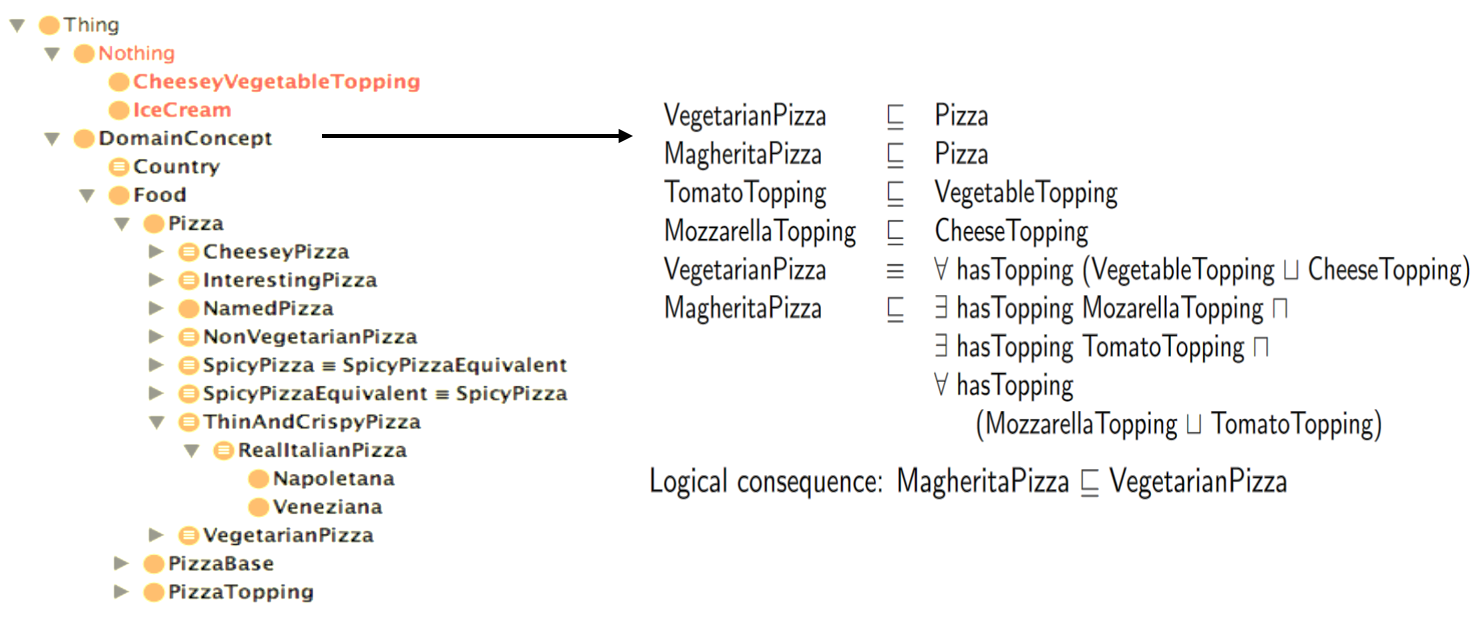
\includegraphics[scale=0.8]{images/reasoning.png}
	\caption{Example of inferencing logical conclusion} 
	\label{fig:pizza1}
	\vspace{-2mm}
\end{figure*}

\subsection{Deductive reasoning} 
It is a basic form of valid reasoning in which the deduction starts with a general statement. Then all the possibilities are checked to reach a specific and logical conclusion. Scientific methods often use deduction to test hypotheses and theories. In deductive inference, we hold a theory, followed by predicting the observations if the theory was correct. Conclusions are also often drawn similar to what we do based on mathematics from a logical syllogism. 
\iffalse
\vspace{-4mm}
{\scriptsize \noindent Example 1: \texttt{`All oncogenes are responsible for cancer; TP53 is a oncogene; therefore, TP53 is responsible for cancer'}. \\
    Example 1: \texttt{`All oncogenes are responsible for cancer; TP53 is a oncogene; therefore, TP53 is responsible for cancer'}. \\
    %Example 1: \texttt{`All oncogenes are responsible for cancer; TP53 is a oncogene; therefore, %TP53 is responsible for cancer'}
    }.\\
\vspace{-4mm}    
\begin{figure}[!ht]
		\centering
		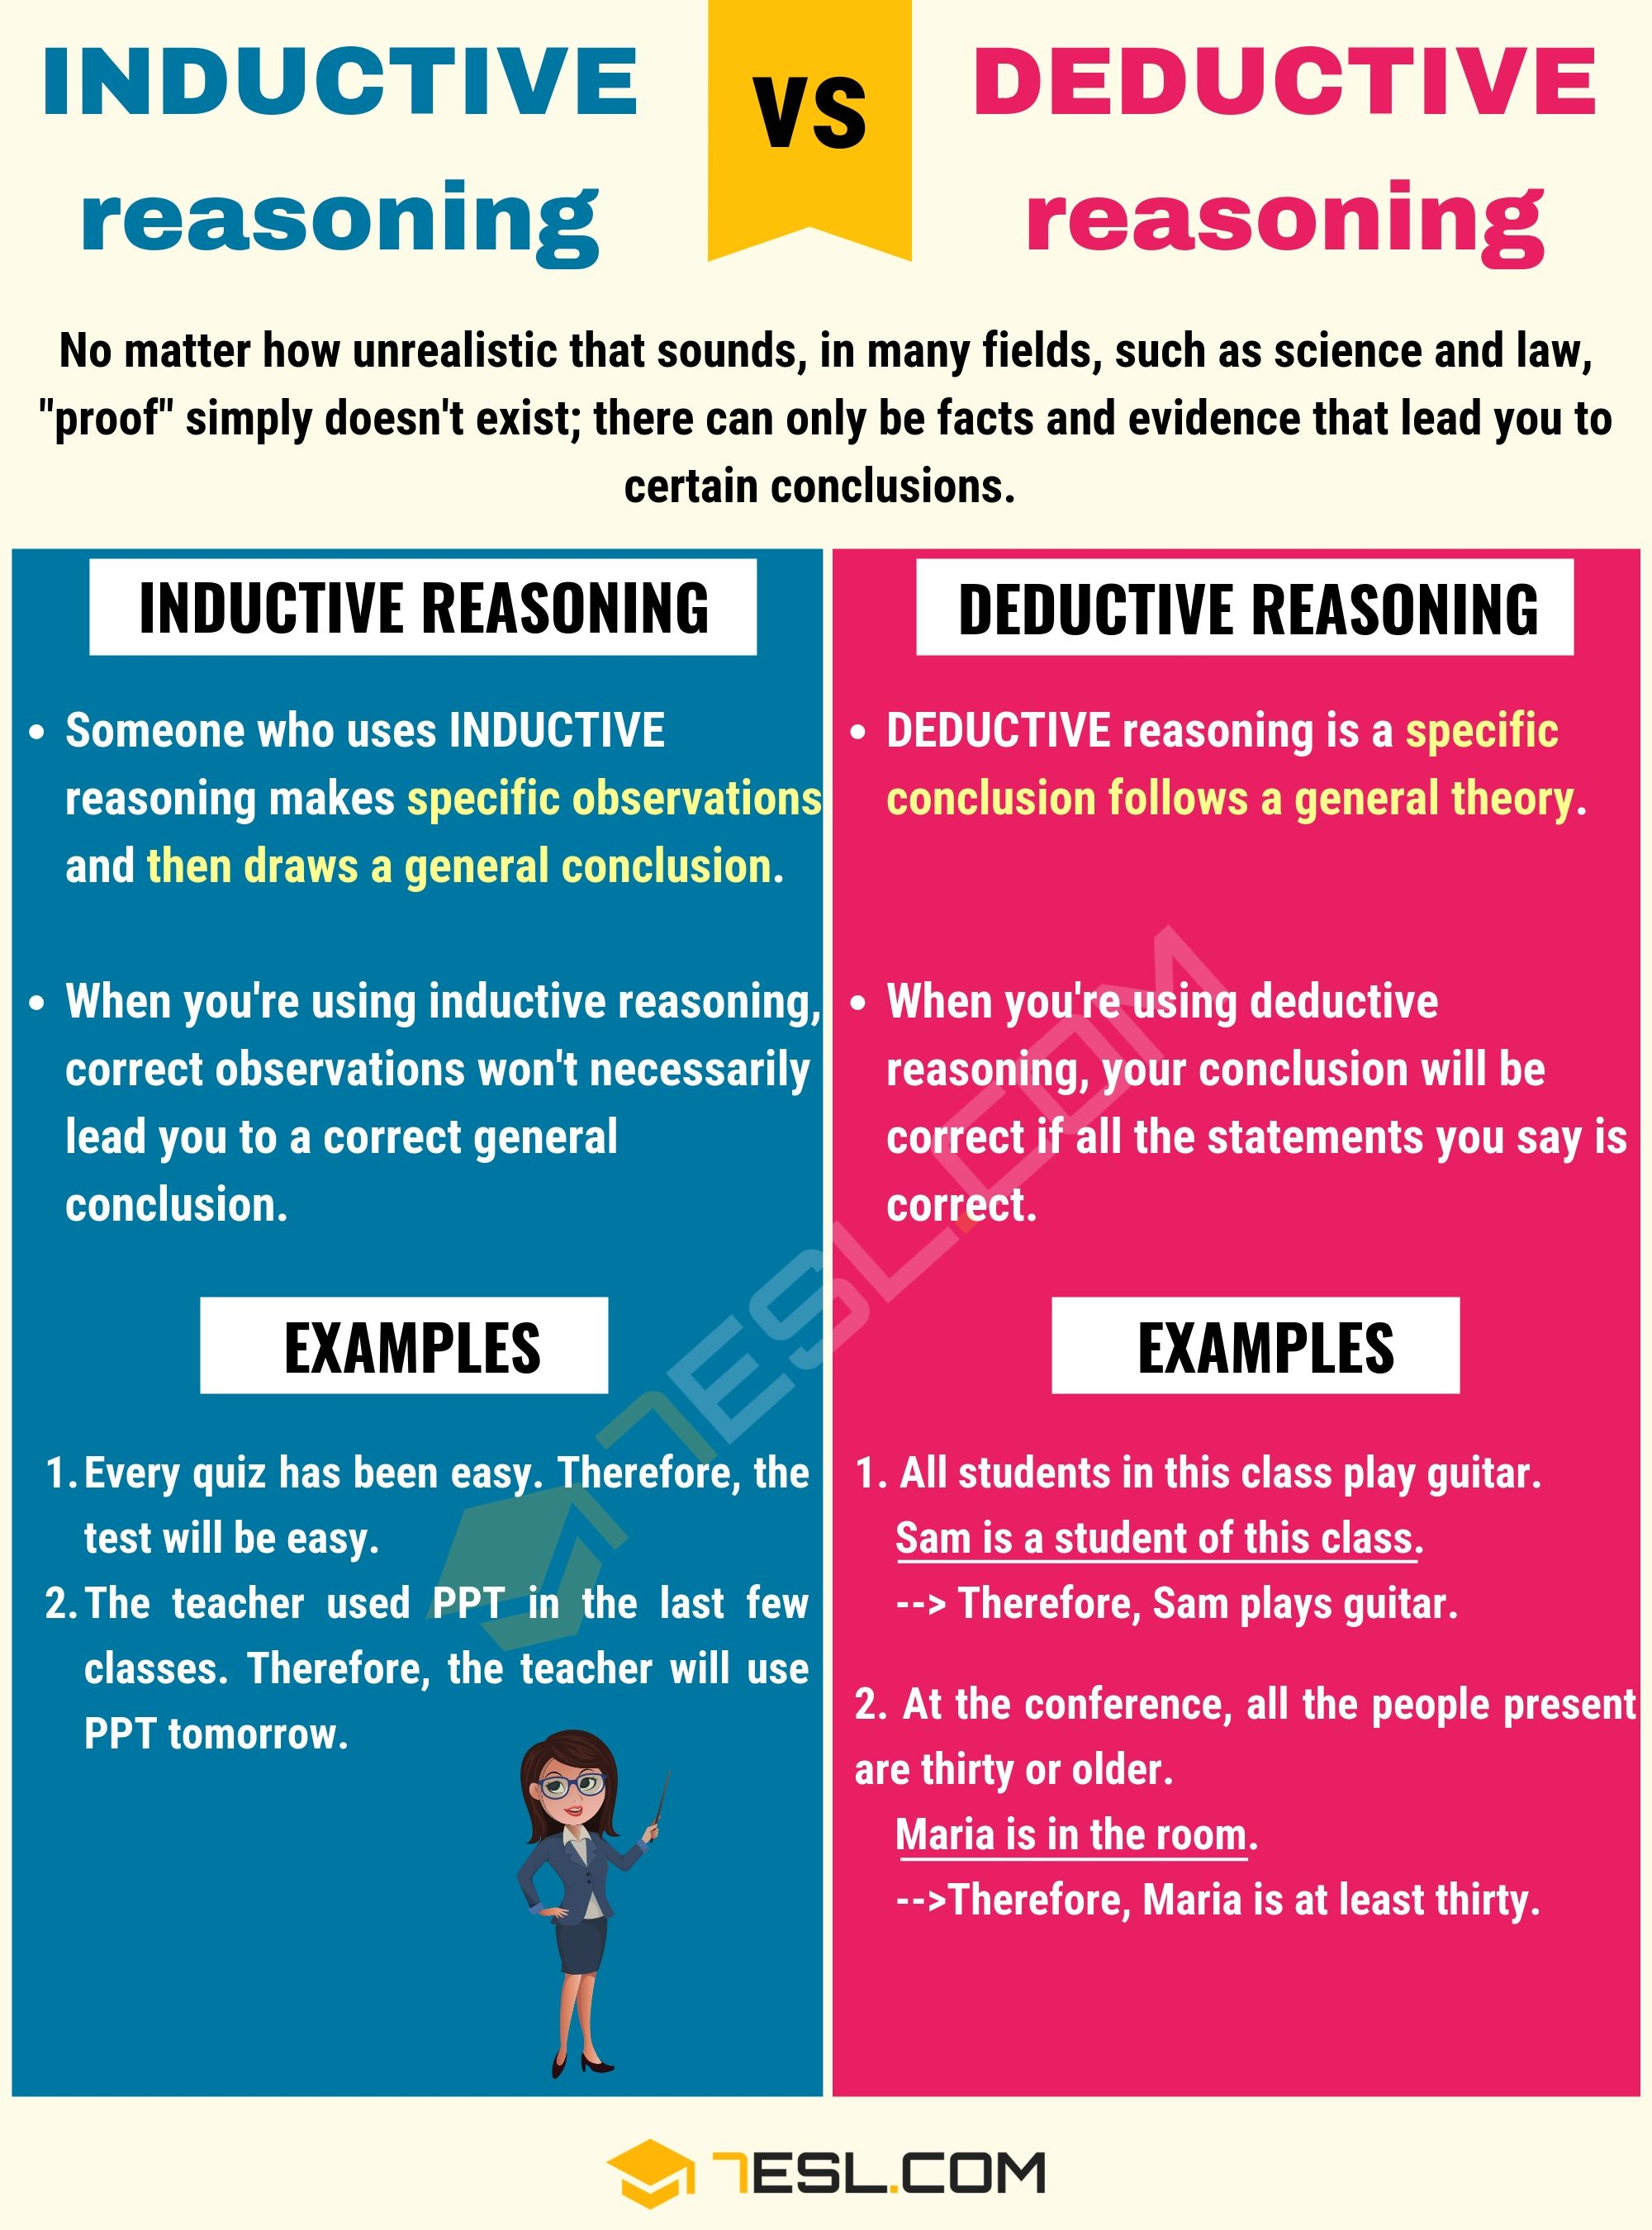
\includegraphics[width=\linewidth]{Inductive-vs-Deductive-Reasoning.jpg}
        \label{fig:pizza}
	\caption{Inductive vs deductive reasoning} 
\end{figure}
\fi 
Deductive reasoning usually involves: a premise, followed by one or more premise, and finally an inference, e.g., \texttt{`All oncogenes are responsible for cancer; TP53 is a oncogene; therefore, TP53 is responsible for cancer'}. When the deductive reasoning is used, the conclusion will be correct if all the statements are correct. 

\subsection{Inductive reasoning} 
Often symbols express lessons we derive inductively from domain knowledge or real-world experience. Inductive reasoning is the opposite of deductive reasoning in which a broad generalizations is made from specific observations or data. In real-life, we make many observations, discern a pattern, make a generalization, and infer an explanation or a theory. Someone who uses inductive reasoning makes specific observations and draws a general conclusion, e.g., `Oncogenes are responsible for cancer, don't apply gene silencing blindly'. 
\iffalse
\vspace{-4mm}
{\scriptsize \noindent Example 1: \texttt{`Oncogenes are responsible for cancer, don't apply gene silencing blindly'}. \\ Example 2: \texttt{`Oncogenes are responsible for cancer, don't apply gene silencing blindly'}}.\\
\vspace{-4mm}
\fi 
The downside of inductive reasoning is that it can follow a false conclusion, even if all of the premises are true in a statement. For example, \texttt{`TCF3 is an oncogene; TCF3 has tumor-suppressor functionality; all oncogenes have tumor-suppressor functionality"}. The conclusion, however, does not follow logically from the statements, because biologically only the proto-oncogenes have such tumor-suppressor functionality.

\section{Methods}\label{chapter_8:mm}
In this section, we discuss the approach for symbolic decision reasoning in detail. The workflow of the overall reasoning method, which is inspired by an XAI system proposed by Giuseppe Futia et al.~\cite{futia2020integration} is shown in \cref{fig:reasoning_wf} and the `Semantic Referee' proposed by Alirezaie et al.~\cite{alirezaie2019semantic}. Further, our approach utilizes the generated rules we explained in \cref{chapter:xai_rules}. We developed an ontology which can enable semantic reasoning for verification of the predictions for relations between diseases and genes. The ontology we introduce here allows the aforementioned reasoning by using different rules which are derived from the ontology itself. Subsequently, the SR would help inferred and validate the matched concepts, enrich with domain knowledge and returns the modified rules before explaining to end users, where the query and reasoning mechanisms over KGs enable interactive and rule-based explanations. 

\begin{sidewaysfigure}
	\centering
	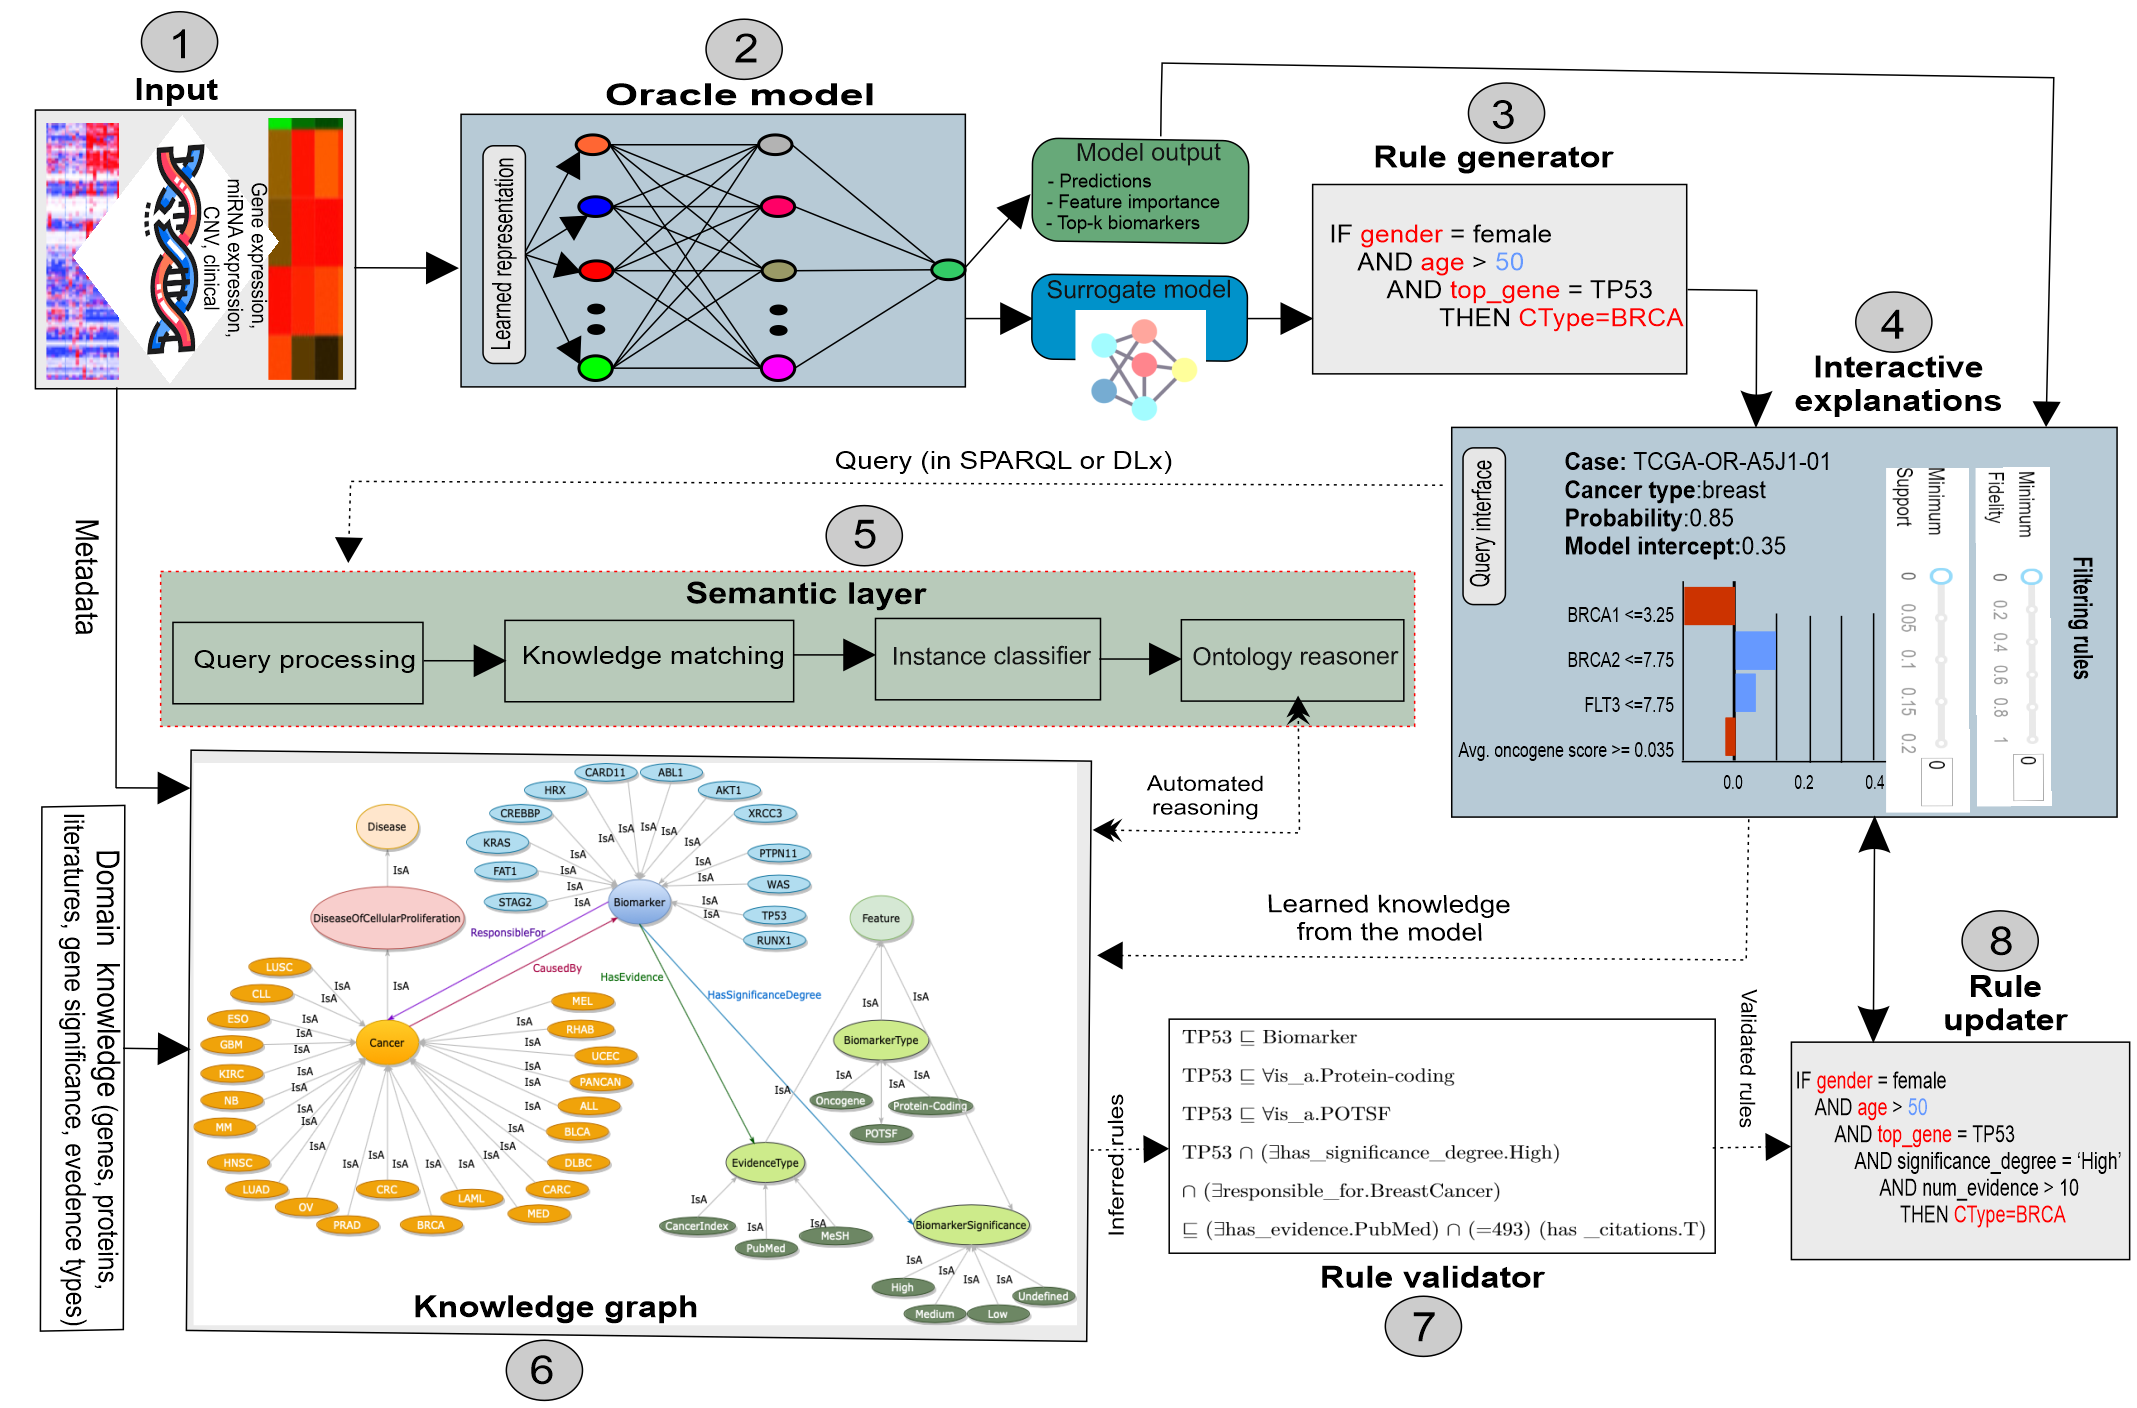
\includegraphics[scale=0.9]{images/reasoning_wf.png}
	\caption{Workflow of the overall reasoning method} 
	\label{fig:reasoning_wf}
	\vspace{-2mm}
\end{sidewaysfigure} 

\hspace*{3.5mm} In a nutshell, a semantic reasoner provides the foundation of the semantic layer, where a reasoner infers and produces new knowledge from existing knowledge from the KB in order to answer interactive queries. 
%\subsection{Problem statement}
%However, to know the global-behaviour and validation of the generated decision rule set,
The goal to acquire knowledge and store it in KB is to provide querying facilities for the end-user in interactive explanation scenario. In a similar, argument, the main reasoning task is query answering. However, in our case the querying is enriched by a rule-based layer. Thus the reasoner takes into account the domain-knowledge represented within the rules while querying. 

\subsection{Problem statement}
Therefore, given a rule list, the knowledge matching module performs matching antecedents with the ontological concepts by applying ontology-based axioms classification. Ontological relations in the form of logic-based axioms are used by reasoning methods to infer both implicit and explicit information~\cite{alirezaie2017ontology}. More formally, given a set of facts $\mathcal{F}$ and a set of rules $\mathcal{R}$, i.e., all the deducible knowledge are computed until no rule is applicable. If the closure of a set of facts $\mathcal{F}$ is the same as $\mathcal{F},$ i.e., $\mathrm{Cl}_{\mathcal{R}}(\mathcal{F})=\mathcal{F}$, then we say that $\mathcal{F}$ is closed under the application of rules or deductively closed~\cite{garoufallou2016metadata}. We hypothesize that a query $Q$~(it could be a query in human language, a SPARQL, or query in DLx format) has an answer within a knowledge base $\mathcal{K}$ if and only if $\mathrm{Cl}_{\mathcal{R}}(\mathcal{F}) \models Q$ where $\models$ refers to the usual first-order entailment~\cite{garoufallou2016metadata}. 

\subsection{Construction of the semantic layer}
Depending on the hierarchy of abstraction, relations between concepts can be more complicated, making it difficult to interpret. However, based on existing concepts, an ontology-based reasoning process is able to retrieve  domain-specific concepts using the subsumption relations between concepts~\cite{alirezaie2019semantic}. Since we already generated the rule set satisfying a certain threshold of minimum support and fidelity, on which we can already perform interactive visual explanations, we focus on the construction of the semantic layer. 

\hspace*{3.5mm} Our semantic layer consists of query processing module, knowledge matching module, instance classifier, and the ontology reasoner. This layer provides an interface between the KG and the rule generator. Since a domain-specific ontology is a mandate, we start with the ontology development in which a set of vocabulary and facts we will embed into. Then we model the ontology as a KG. The KG would contain domain-specific knowledge about cancer genomics and composed of three main components:

\vspace{-2mm}
\begin{itemize}[noitemsep]
    \item \textbf{Vocabulary} - containing knowledge about concepts and relations w.r.t cancer genomics. 
    \item \textbf{Rules} - representing rules~(we treat it the rule-base) that encode generic knowledge. 
    \item \textbf{Facts} - containing factual knowledge about cancer genomics subjects.
    \vspace{-4mm}
\end{itemize}

\subsection{Ontology development}
Ontologies classify things and define more specific relations and attributes, where entities can be specifically classified and thus become an
instance of one or more classes. In conjunction, restrictions can now be expressed in order to develop a more consistent knowledge model. Ontologies are also used to take advantage of inference mechanisms. Since the semantic annotations are typically based on predefined concepts w.r.t. biological entities, a domain-specific ontology is required to perform ontological reasoning. Annotations also help enrich the KG with domain knowledge about relations between concepts to facilitate more complex and elaborate reasoning. In our approach, instead of building a new ontology from scratch\footnote{Part of the ontology was developed by Lina Teresa Molinas Comet \& Suchanda Bhattacharyya for \url{http://xai.fit.fraunhofer.de:5000/}}, we build it in the form of KG based on several existing ontologies. We reuse existing and rich ontologies to represent domain knowledge about human diseases, annotations about genes, cancers, mutations, metadata ~(i.e., labels and provenance), and corresponding evidences from scientific literature. 

\subsubsection{Ontology modelling}
As a ground basis, we used the ontology of gene ontology~(GO), human phenotype ontology, disease ontology, genes and genomes~(OGG)\footnote{\url{https://bioportal.bioontology.org/ontologies/OGG/?p=classes&conceptid=root}}, and the human disease ontology~(DOID)\footnote{\url{https://bioportal.bioontology.org/ontologies/DOID/?p=classes&conceptid=root}}. Our decision was made based on the fact that those two ontologies model entities about genes and genomes, and human diseases respectively. We inherited the metadata of the entities from both ontologies. Additionally, we complemented the metadata for the entities by adding information from two other resources, i.e., TumorPortal\footnote{\url{http://www.tumorportal.org}} and the cancer genetics website\footnote{\url{http://www.cancer-genetics.org/genes_a.htm}}. 

\hspace*{3.5mm} We reused semantic concepts from several sources to model our ontology, which can reflect the structural aspects of the connection between biomarkers~(e.g. oncogenes, protein-coding) and cancer types~(e.g. breast cancer, colorectal cancer). We aim it using this ontology for inferring rules which can be used as a reasoning engine towards simple querying to get domain-specific information about a biomarker responsible for certain cancer types. Moreover, the types of queries that can be answered based on the ontology reasoner are also extended to the evidence supporting a specific relation, as well as the degree of significance of a gene for certain cancer types. 

\paragraph{Human disease ontology:} \hspace*{-2.5mm} as an initial resource we used the DOID, which provides a general schema describing human related diseases. The DOID has been developed by `BioPortal', which provides a comprehensive hierarchical controlled vocabulary for human disease representation, in biomedical resources, health, human, neurologic disease, and neurological disorder categories. The ontology is organized in classes and sub-classes, where the most general class is \texttt{doid:Disease}, which contains different subclasses for each general group of diseases which in turn contain other specific sub-classes like diseases. The relation between entities are expressed with different axioms. 
\hspace*{3.5mm} The whole structure of the DOID ontology is not inherited since it contains many sub-groupings that are not crucial for our requirement. Instead, we focused on the sub-classes `disease of cellular proliferation' and `disease of anatomical entity', and more specifically in the classes containing `cancer' related facts about cancer types. \Cref{fig:oncoontology14} shows the hierarchical relation between between classes and sub-classes. \\ 

\vspace{-4mm}
{\scriptsize \noindent doid:Disease$\sqsubseteq$owl:Thing \\
doid:DiseaseOfCellularProliferation$\sqsubseteq$ doid:Disease\\
doid:Cancer$\sqsubseteq$ doid:DiseaseOfCellularProliferation\\
doid:DiseaseOfAnatomicalEntity$\sqsubseteq$ doid:Disease\\ 
doid:BreastCancer$\sqsubseteq$doid:BreastDisease$\sqsubseteq$doid:ThoracicDisease$  \sqsubseteq$doid:DiseaseOfAnatomicalEntity.} \\

\vspace{-4mm}

\begin{figure*}
	\centering
	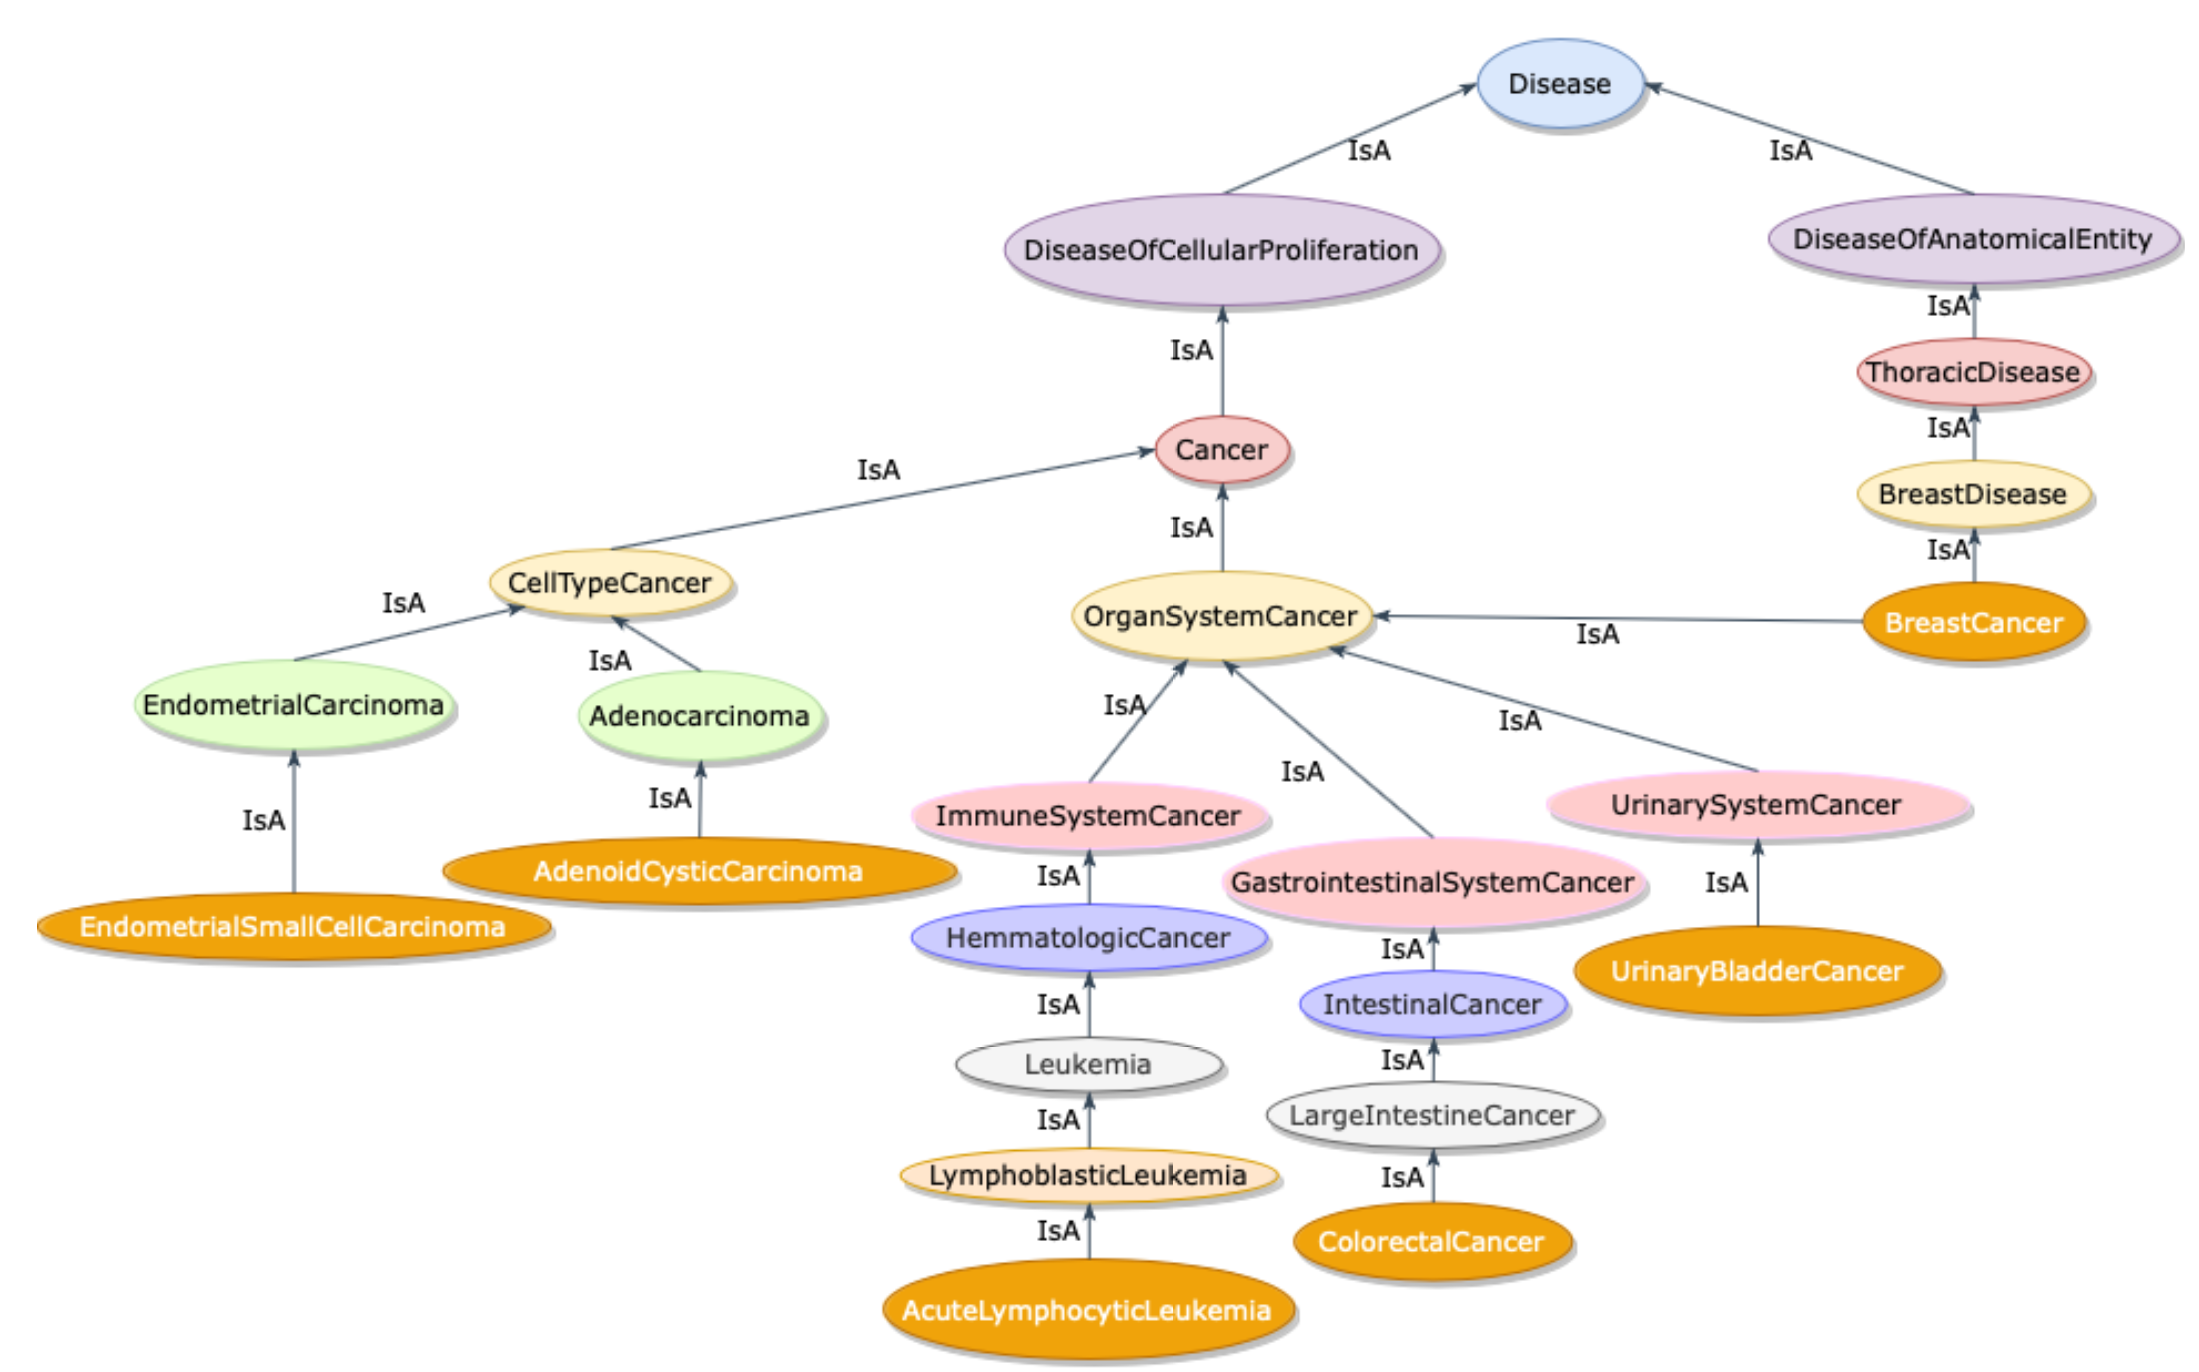
\includegraphics[scale=0.5]{images/do.png}
	\caption{High-level view of some part of the DOID ontology} 
	\label{fig:oncoontology14}
	\vspace{-2mm}
\end{figure*}

\hspace*{3.5mm} Each class in the DOID ontology is described with annotations indicating different properties of that object. For example, the annotation `prefLabel' indicates the name of the object, but in addition the annotation `has\_exact\_synonym' indicates the other names with which that object is known in other ontologies. We inherited all the object properties of the entities, namely cancer types.

\paragraph{Ontology of genes and genomes:} \hspace*{-2.5mm} to map diseases with the responsible genes associated with, we used the OGG in which we model the properties of the biomarkers. The OGG ontology uses a hierarchical structure similar to the DOID ontology. However, we focus on the entities under the class `gene of Homo sapiens' which describe genes that are present in humans. It is important to mention that we just inherited the annotations of the properties for each biomarkers~(e.g., gene), such that the gene properties related to certain cancer types were only extracted. \Cref{fig:ogg_ontology} shows the hierarchical relation between classes and sub-classes.\\

\vspace{-4mm}
{\scriptsize \noindent ogg:DiseaseOfCellularProliferation $\sqsubseteq$ doid:Disease\\
ogg:Cancer$\sqsubseteq$doid:DiseaseOfCellularProliferation\\
doid:DiseaseOfAnatomicalEntity$\sqsubseteq$doid:Disease\\
ogg:BRCA1$\sqsubseteq$ogg:ProteinCodingGeneOfHomoSapiens$\sqsubseteq$ogg:GeneOfHomoSapiens$\sqsubseteq$ ogg:Gene$\sqsubseteq$ogg:MaterialEntity$\sqsubseteq$ ogg:Entity.}\\

\vspace{-2mm}
\begin{figure*}
	\centering
	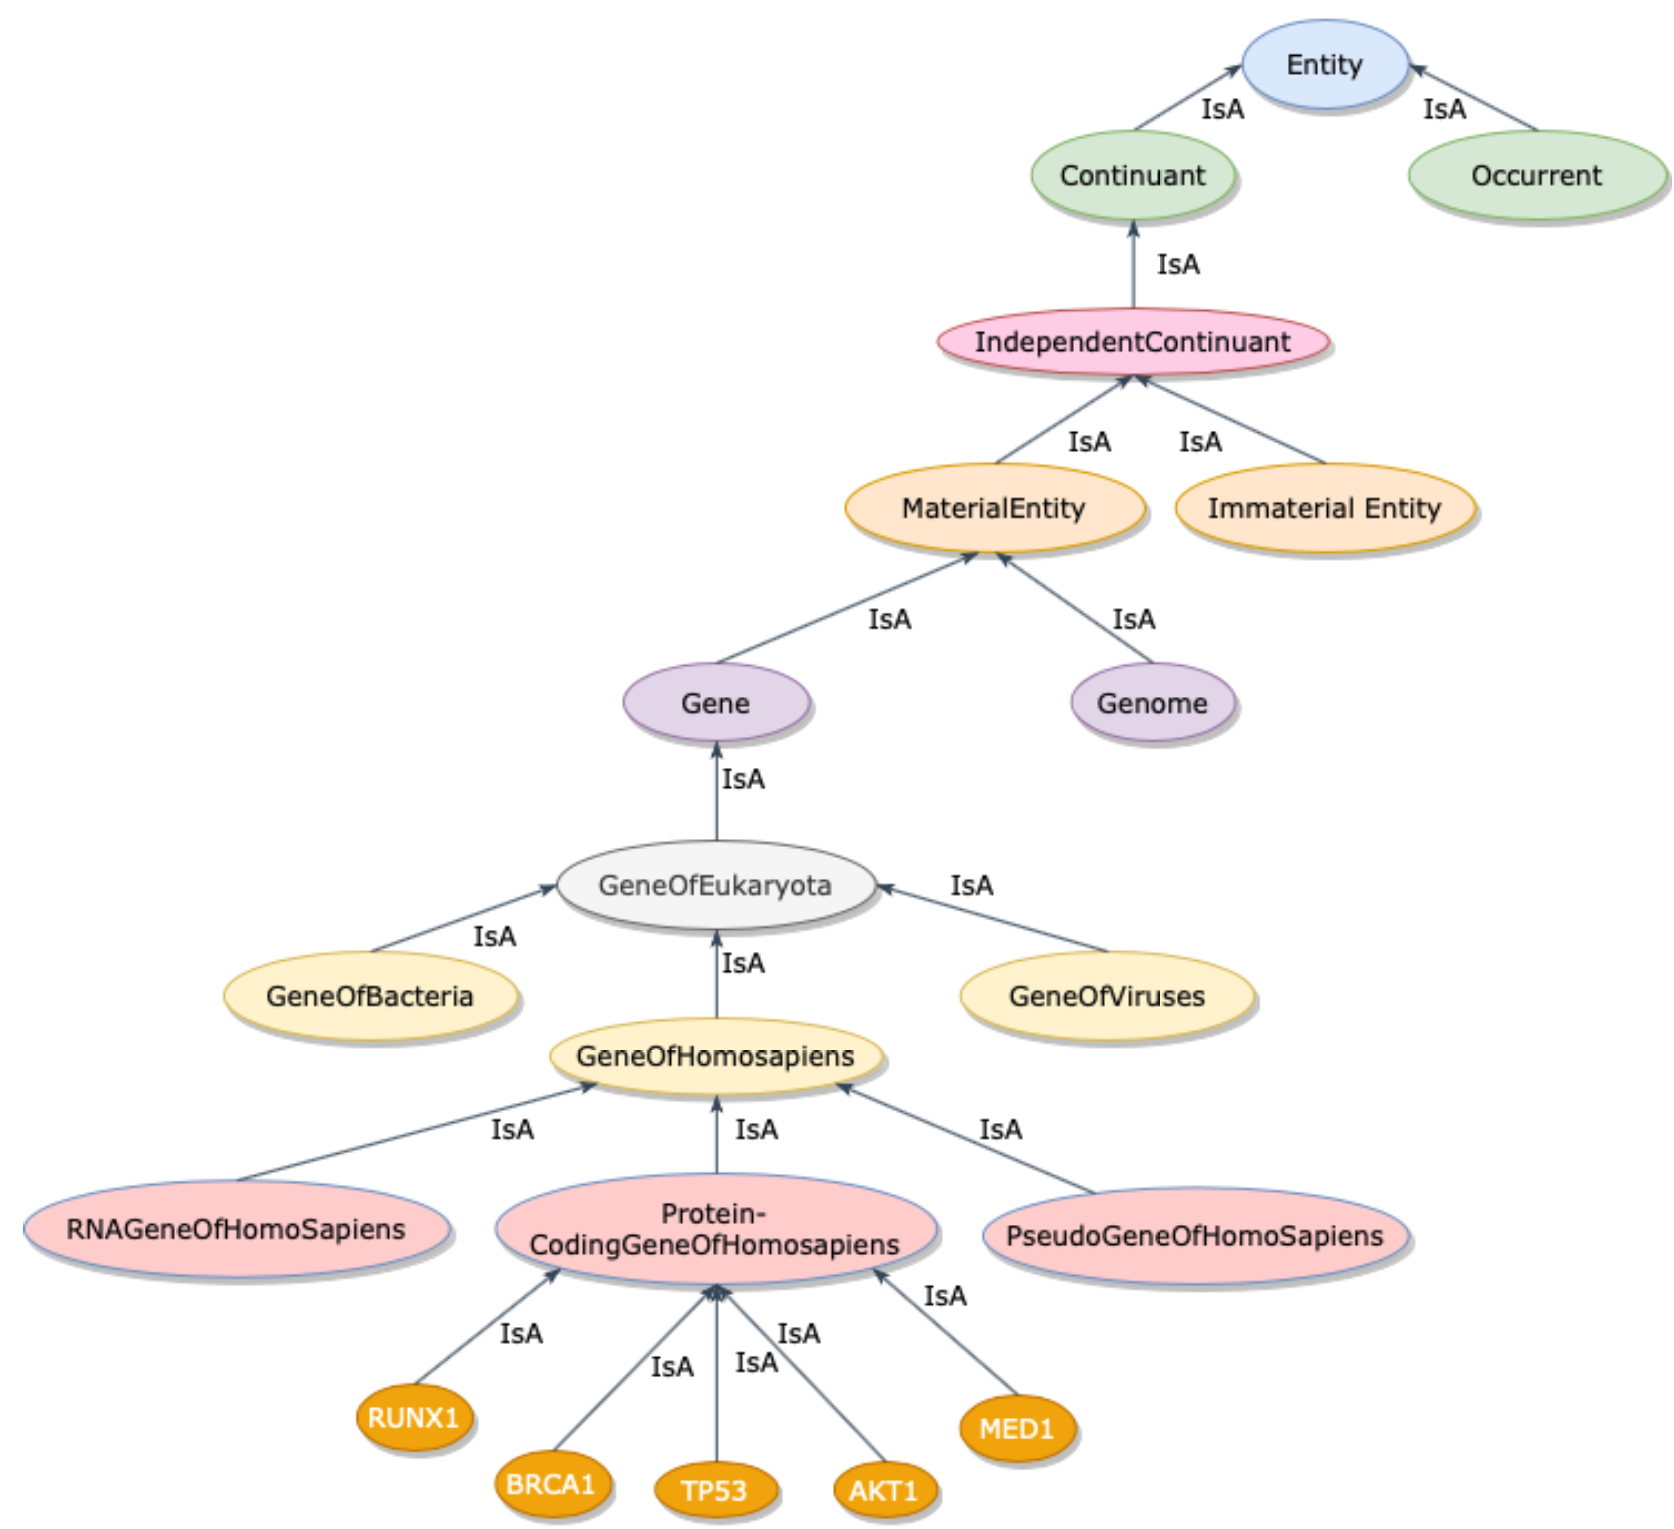
\includegraphics[scale=0.5]{images/go.png}
	\caption{Partial high-level view of the OGG ontology} 
	\label{fig:ogg_ontology}
	\vspace{-2mm}
\end{figure*}

\vspace{-2mm}
\hspace*{3.5mm} Each entity and class is annotated with properties ranging from the name of the entity `preferred name', to the definition, and the alternatives terms `alternative term' used to identify a particular entity. We inherited all the properties for each entity in our new ontology.

\begin{figure*}
	\centering
	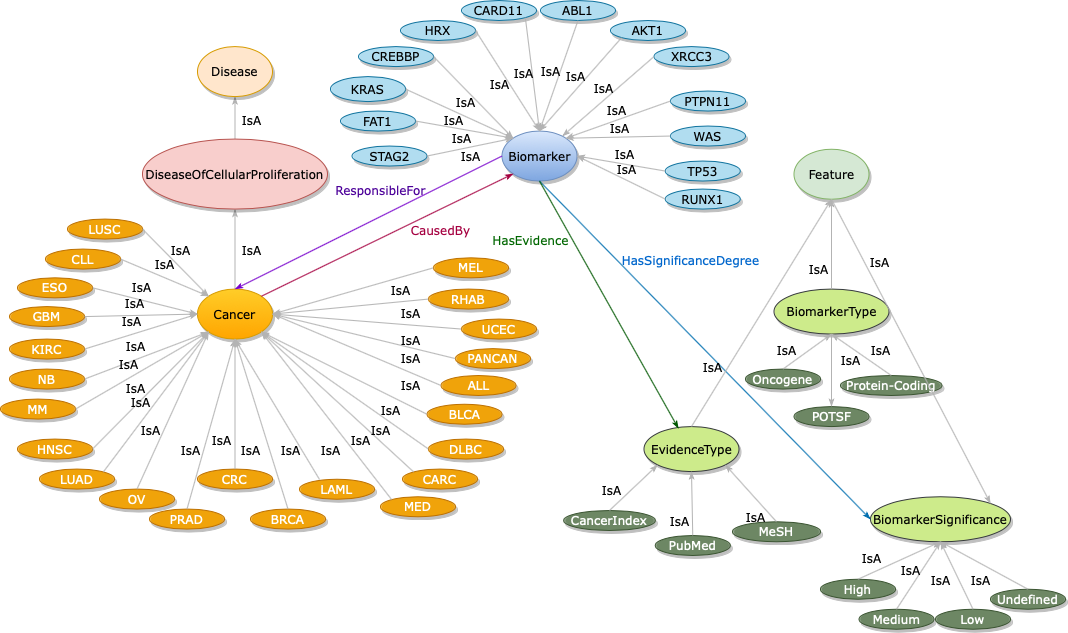
\includegraphics[width=0.8\linewidth,height=60mm]{images/diagram_general_view.png}
	\caption{High-level view of the ontology} 
	\label{fig:main_ontology}
\end{figure*}

\paragraph{Disease ontology, breast cancer ontology, and cancer genetics web:} \hspace*{-2.5mm} the DO is a standardized ontology for human disease, which aims to provide consistent, reusable and sustainable descriptions of human disease terms, phenotype characteristics, and medical vocabulary disease concepts. DO semantically integrates disease and medical vocabularies via cross mapping of DO terms from MeSH, ICD, NCI, SNOMED, and OMIM. The BCO from EBI provides the domain knowledge about breast cancer, which is also a good source of carcinogenics to understand the relations of different biological entities for breast and other cancer. Provides an integrated information from several data source and analysis of the literature using data from PubMed and CancerIndex.org. Further, it also provides and integrated view of the latest research abstracts relating to genes, proteins and cancer.  

\begin{figure*}
	\centering
	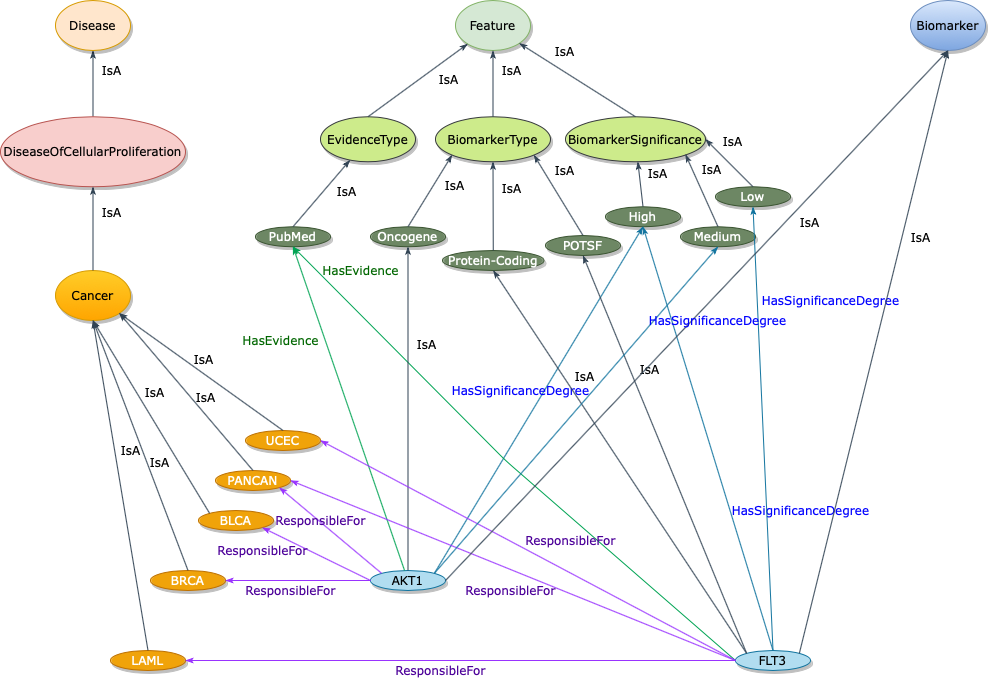
\includegraphics[width=0.8\linewidth,height=65mm]{images/GeneralRelations-Ontology.png}
	\caption{High-level view of the relations in the ontology}
	\label{fig:main_ontology_relations}
	\vspace{-4mm}
\end{figure*}

\hspace*{3.5mm} Our decision was made based on the fact that those two ontologies model entities about genes and genomes, and human diseases respectively. We inherited the metadata of the entities from both ontologies. Besides we enriched our ontology with knowledge from mouse genome informatics~(MGI) that provides genomic data to study human disease, while the TumourPortal provides annotations about genes, cancers, and DNA mutation. Additionally, we complemented the metadata for the entities by adding information from two other resources, namely the TumorPortal and the cancer genetics website. We also integrated knowledge from Tumor Portal website from which we took information regarding the significance degree of the genes which are significantly mutated for some cancer types. Additionally to the entities and their annotations, based on the DOID and OGG ontologies, we complemented the structure and information available in our ontology by adding the information of the significance degree of a gene as a property. 

\begin{figure*}[h]
	\centering
	\begin{subfigure}{0.48\linewidth}
	\centering
		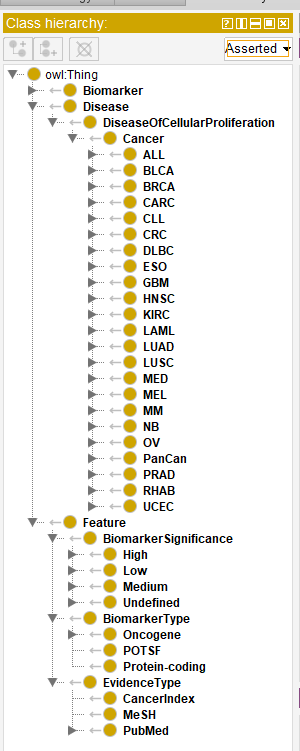
\includegraphics[width=0.55\linewidth,height=70mm]{images/OncoReferee.png}
		\caption{High-level view of the ontology}
        \label{fig:main_ontology_pro_view}
	\end{subfigure}
	\begin{subfigure}{0.48\linewidth}
		\centering
		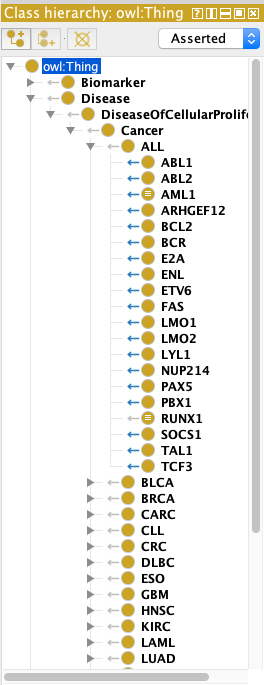
\includegraphics[width=0.55\linewidth,height=70mm]{images/biomarker_view_2.png}
		\caption{Properties of an entity in the disease class}
        \label{fig:diseases_class}
	\end{subfigure}
	\begin{subfigure}{.48\linewidth}
		\centering
		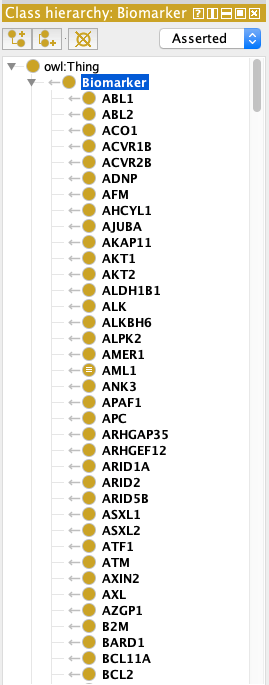
\includegraphics[width=0.55\linewidth,height=70mm]{images/biomarker_view.png}
		\caption{Biomarker class for different cancer types}
        \label{fig:annotations_for_genes}
	\end{subfigure}
	\iffalse
	\begin{subfigure}{0.48\linewidth}
		\centering
		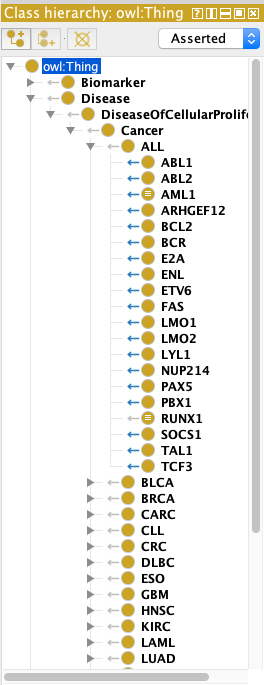
\includegraphics[width=0.55\linewidth,height=70mm]{images/biomarker_view_2.png}
		\caption{Disease subclasses to corresponding cancer types}
        \label{fig:diseases_sub_class}
	\end{subfigure}
	\fi 
	\caption{Hierarchical view of the biomarker and disease class} 
	\label{fig:property_enrich_annotations_for_genes}
	\vspace{-4mm}
\end{figure*}

\subsubsection{Entity relations} 
We map all protein identifiers to Entrez gene identifiers and use these to represent both genes, proteins, and other biological entities. We use PubChem identifiers to represent chemicals and we map UMLS identifiers associated with DO using mappings provided by DO. We further map UMLS identifiers associated with side effects in SIDER to HPO identifiers using mapping between UMLS and HPO. We treat biological entities such as types of proteins, diseases, or chemicals, as instances in the knowledge graph. Classes from the DO are also treated as instances. Moreover, we included  the relation between a specific gene and one or more diseases. There are 3 main classes, which allow us to express the relation between entities. The general structure of the ontology is shown in \cref{fig:main_ontology}, while the hierarchical relations between the different classes and subclasses in the ontology are depicted as follows: \\

\vspace{-4mm}
{\scriptsize \noindent biomarker$\sqsubseteq$owl:Thing \\
BRCA1$\sqsubseteq$biomarker\\
Disease$\sqsubseteq$owl:Thing\\
BRCA$\sqsubseteq$Cancer$\sqsubseteq$DiseaseOfCellularProliferation$\sqsubseteq$Disease.}\\
\vspace{-4mm}

\subsubsection{Cancer specific biomarkers}
\Cref{fig:main_ontology_pro_view} shows the hierarchical view of the biomarker class, where we included all the biomarkers, particularly, genes related to all the cancer types we consider in this ontology. The possible sub-classes of `BiomarkerSignificance' is then defined as HIGH, MEDIUM, and LOW based on the annotations provided by the TumorPortal\footnote{\url{http://www.tumorportal.org/tumor_types?ttype=PanCan}}. Further, each entity belonging to the class biomarker is annotated with all the information of properties available in the OGG ontology, as shown in \cref{fig:ogg_ontology}. Besides, we included the number of scientific articles as an evidence associated with certain genes, which is shown in \cref{fig:biomarker_subclass}.

\subsubsection{Enriching disease specific knowledge}
The `Disease' class consists of a subclasses named  `DiseaseOfCellularProliferation' under which there is another sub-class called `Cancer'. Under the class Cancer we included all the cancer types we are interested in, and which are labeled with their well-known abbreviations, e.g., BRCA for breast cancer. \Cref{fig:diseases_class} shows the structure of the class disease and its subclasses. As we mentioned, for the entities in the class disease we also inherited the object properties from the DOID ontology and included them as annotations. 

\iffalse
\begin{figure*}[h]
	\centering
	\begin{subfigure}{.48\linewidth}
		\centering
		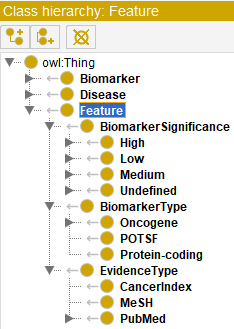
\includegraphics[width=0.6\linewidth,height=60mm]{images/feature_class.png}
		\caption{Biomarker class}
        \label{fig:feature_class}
	\end{subfigure}
	\begin{subfigure}{0.48\linewidth}
		\centering
		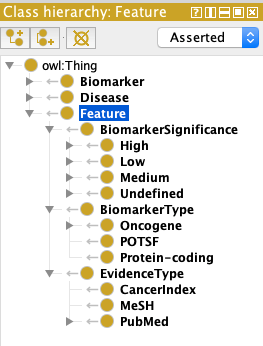
\includegraphics[width=0.6\linewidth,height=60mm]{images/feature1.png}
		\caption{Biomarker subclass}
        \label{fig:biomarker_subclass}
	\end{subfigure}
	\caption{Annotations and relations between entities in the biomarker class and subclass}
	\label{fig:biomarker_class_subclass}
	\vspace{-2mm}
\end{figure*}
\fi 

\begin{figure*}[h]
	\centering
		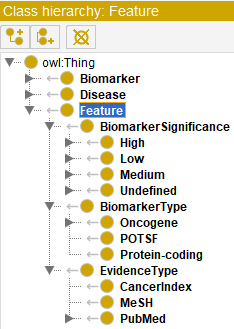
\includegraphics[width=0.3\linewidth,height=60mm]{images/feature_class.png}
        \label{fig:biomarker_subclass}
	\caption{Annotations and relations between entities in the biomarker class and subclass}
	\vspace{-2mm}
\end{figure*}

%\subsubsection{Enriching gene specific evidence}
\hspace*{3.5mm} Further, we included the class `Feature' to express the relation between a disease and the responsible genes associated with it. More specifically, we indicate the significance degree of a particular gene, regarding a disease. Besides, we included biomarker type and the evidence type information. Furthermore, since depending on the types gene biomarkers can be categorized as `Oncogene', `Protein-coding', and `POTSF', we considered these as the subclasses of `BiomarkerType'. As many as 83 POTSF genes identified by Libing Shen et al.~\cite{POSTF} through database search and literature annotation are used to enrich the list. 

\begin{itemize}[noitemsep]
    \item \textbf{Proto-oncogenes with tumor-suppressor function} - some genes have both oncogenic and tumor-suppressor functions, i.e., they have both oncogenic and tumor-suppressor functionality~\cite{POSTF}.
    \item \textbf{List of POTSF genes} - BRCA1, CAMTA1, CBFA2T3, CDX2, CREB3L1, CREBBP, DDB2, DNMT1, DNMT3A, ETV6, EZH2, FOXA1, FOXL2, FOXO1, FOXO3, FOXO4, FOXP1, FUS, IRF4, KLF4, KLF5, NCOA4, NOTCH1, NOTCH2, NOTCH3, NPM1, NR4A3, PAX5, PML, PPARG, RB1, RUNX1, SMAD4, STAT3, TCF3, TCF7L2, TP53, TP63, TRIM24, WT, ZBTB16, BCR, CHEK2, EPHA1, EPHA3, EPHB4, FLT3, MAP2K4, MAP3K4, MST1R, NTRK3, PRKAR1A, PRKCB, SYK, ARHGEF12, BCL10, BRCA2, CBL, CDC73, CDH11, CDKN1B, DCC, DDX3×, DICER1, FAS, FAT1, GPC3, IDH1, IKZF2, LIFR, NF2, NUP98, PHF6, PTPN1, PTPN11, RHOA, RHOB, SH2B3, SLC9A3R1, SOCS1, SPOP, SUZ12, WHSC1L1~\cite{POSTF}. 
\end{itemize}

\hspace*{3.5mm} PubMed, MeSH, and CancerIndex are considered as the source of the evidence. \Cref{fig:biomarker_subclass} shows the general structure of the `Feature' class. These features~(in terms of annotations and object properties) are used to indicate the relation between entities from different classes, as shown in \cref{fig:biomarker_subclass}, which in turn annotations allow the rules generation. 

\subsection{Semantic layer}
As already stated, our semantic layer, consists of four components: query processing module, knowledge matching module, instance classifier, and the ontology reasoner. The ontology represented as a RDF KG consists of 31,034 triples including data, ontologies, and formal representation annotations. The semantic layer provides an interface between the KG and the rule generator. We provide the details of each component in this sub-section.

\subsubsection{Query processing}
Having extracted a set of concepts from the decision rules, we relate them to the KG in SPARQL or DLx query format. For the former, concepts are stored as RDF triples and queried via SPARQL endpoint. For the latter, we query via Prot{\'e}g{\'e}\footnote{An open-source tools to construct domain models and knowledge-based applications with ontologies, Link: \url{https://protegewiki.stanford.edu/wiki/Main_Page}} DLx query view. 
%\subsubsection{Query formulation}
With all concepts mapped to KB entities, the next step is forming queries in SPARQL or DLx formats, depending on the question template. 
A human agent or end users like clinicians/doctors may require to formulate the query in a convenient way. However, for the simplicity, we focus on the DLx queries, albeit SPARQL is definitely our outlook for better the expressivity. The next step is then to generate answers according to the results of the queries, where the reasoner searchers concepts in the KG that are already classified w.r.t entity types, which we use to give ``logical reasons" as to how the answer is generated. Especially for questions requiring external knowledge, the predicates and entities on the path give a better understanding of how the relationships are established between the concepts from the rule and and KB concepts. 

\subsubsection{Instance classification and reasoning}
In order to perform reasoning in forward chaining in presence of rules, the reasoner applies all the rules in the rule-base on the set of facts in the factual part then query the KG in a classical manner.
In many cases, a set of facts $\mathcal{F}$ may contain contradictory knowledge, giving inconsistencies. We say that a set of facts is inconsistent $iff$  $\mathrm{Cl}_{\mathcal{R}}(\mathcal{F})$ triggers a negative constraint~\cite{garoufallou2016metadata}. However, for the simplicity, we assume that our rule-base does not contain contradictory rules. 

\hspace*{3.5mm} We have two distinct types of entities: biological entities and classes from biomedical ontologies that provide background knowledge about entities. Ontology-based annotations are expressed by asserting a relation between the instance, e.g., a gene and cancer types and an instance of the ontology class. For example, we express the information that the gene $AKT1$ has the GO association \texttt{GO:0000060} by two axioms \texttt{hasGOAssociation(AKT1,$f_1$)} and \texttt{instanceOf($f_1$, GO:0000060)}, where $AKT1$ and $f_1$ are instances, \texttt{GO:0000060} is a class \url{http://purl.obolibrary.org/obo/GO\_0000060} in GO, \texttt{hasGOAssociation} is an object property, and \texttt{instanceOf} is the \texttt{rdf:type} property in OWL standard. 

\hspace*{3.5mm} In our KG, we assign each instance $f_i$ a unique IRI. We follow OWL2 EL standard for representing KGs and utilize different reasoners such as Pellet, HermiT, and ELK for automated reasoning over them. OWL2 EL that supports basic inferences over ontological class hierarchies and object properties, can infer the classification of instances, via  the class descriptions, class axioms, and object property axioms~\cite{alshahrani2017neuro}: 

\begin{itemize}[noitemsep]
\vspace{-4mm}
    \item \textbf{Class description} - class intersection $(A \sqcap B)$, existential quantification $(\exists r . A),$ limited enumeration using a single instance $\left(\left\{x_{i}\right\}\right)$. 
    \item \textbf{Class axioms} - $E_{1}$:$E_{2}$ indicates entity $E_{1}$ is an instance of class $E_{2}$, subclass $(A \sqsubseteq B)$\footnote{Means concept $A$ is subsumed by concept $B$}, equivalent class $(A \equiv B)$, disjointness $(A \sqcap B \sqsubseteq \perp)$. 
    \item \textbf{Object property axioms} - sub-property $(r \sqsubseteq s)$, property chains $(r \circ s \sqsubseteq q)$, equivalent property $(r \equiv s)$, transitive properties $(r \circ r \sqsubseteq r)$, reflexive properties. 
    \vspace{-4mm}
\end{itemize}

\hspace*{3.5mm} We use the Pellet reasoner to deductively close the KG, i.e., we deductively close our KG w.r.t. the OWL2 EL profile. The $\mathcal{KG}$ would be deductively closed $iff$ for all $\phi$ s.t. $\mathcal{KG} \models \phi, \phi \in \mathcal{KG}$. Although the deductive closure of a knowledge is countably infinite, we assume it is finite for our case. Subsequently, we add only inferences that can be represented explicitly as edges between named individuals and classes~(i.e., entities that are explicitly named) in the $\mathcal{KG}$ s.t. for all instances $x_{i}, x_{j} \in \mathcal{KG}$ and object properties $r \in \mathcal{KG}$, if $\mathcal{KG} \models r\left(x_{i}, x_{j}\right)$, then $r\left(x_{i}, x_{j}\right) \in \mathcal{KG} ^{\models}$. Furthermore, for all named classes $C \in \mathcal{KG}$ and instances $x \in \mathcal{KG}$, if $\mathcal{KG}=\mathrm{C}(x)$, then $C(x) \in \mathcal{KG} ^{\pm}$. Finally, relations between classes are inferred by adding subclass axioms to the inferred graph, s.t. for any class $C, D \in \mathcal{KG}$, if $\mathcal{KG} \models C \sqsubseteq D$, then $C \sqsubseteq D \in \mathcal{KG}^{\pm}$. 

\section{Evaluations}\label{chapter_8:results}
In this section, we discuss the evaluation results, both quantitatively and qualitatively. Besides, a comparative analysis with state-of-the-art approaches is provided. 

\subsection{Experiment setup}
We used Prot{\'e}g{\'e} 5.5.0 is used for the reasoning, DLx querying, and DL rule generations with Pellet, RLK, and HermiT reasoners. 
%The detail information including versions are shown in \cref{fig:plugins_info}. 
However, ELK does not support object all values from axioms, while HermiT gave some inconsistent~(giving different number of rules). Therefore, we report the rules generated with Pellet only. The inferred rules based on the reasoning are expressed using DLx format. 

\subsection{Query benchmarks}
Below we provide a few questions in human language~(NLQ) and in DLx query~(DLQ) format. The answers based on different reasoners can be found in appendix. However, as shown in in \cref{fig:sample_q_a}, the answer of NLQ ``List of all biomarkers which are classified POTSF and responsible for breast cancer answered" against the DLQ ``Biomarker and responsible\_for some BRCA and is\_a only POTSF" by the Prot{\'e}g{\'e} is understandable but not clear how the reasoner derives such answer. Therefore, in the next subsection, we derive corresponding rule for individual biomarker. 

\iffalse
\begin{sidewaystable*}
    \caption{Example of gene expression samples based on oncogenes}
    \label{table:nlq_dlq}
    \vspace{-6mm}
    \begin{center}
        \scriptsize
        \begin{tabular}{l|l}
            \hline
            \rowcolor{Gray}
            \textbf{NLQ} & \textbf{DLQ} \\\hline  
                What is BLCA? & BLCA \\\hline
                What is Cancer? & Cancer \\\hline
                List of all biomarkers? & Biomarker \\\hline
                Which biomarkers have PubMed evidence associated? & has\_evidence \textcolor{blue}{some} PubMed \\\hline
                List of Oncogene, POTSF, and Protein-Coding biomarkers? & Biomarker \textcolor{green}{and} is\_a only Oncogene \textcolor{green}{and} is\_a only POTSF \textcolor{green}{and} is\_a only Protein-coding \\\hline
                List of Oncogene biomarkers responsible for Medulloblastoma with evidence? & Biomarker \textcolor{green}{and} responsible\_for \textcolor{blue}{some} MED \textcolor{green}{and} is\_a only Oncogene \textcolor{green}{and} (has\_evidence \textcolor{blue}{some} PubMed \textcolor{red}{or} has\_evidence \textcolor{blue}{some} CancerIndex \textcolor{red}{or} has\_evidence \textcolor{blue}{some} MeSH) \\\hline
                List of Oncogene, POTSF, and Protein-coding biomarkers responsible for breast cancer? & Biomarker \textcolor{green}{and} responsible\_for \textcolor{blue}{some} BRCA \textcolor{green}{and} is\_a only Oncogene \textcolor{green}{and} (is\_a only POTSF \textcolor{red}{or} is\_a only Protein-coding) \\\hline                
                List of Oncogene biomarkers responsible for breast cancer? & Biomarker \textcolor{green}{and} responsible\_for \textcolor{blue}{some} BRCA \textcolor{green}{and} is\_a only Oncogene \\\hline
                List of POTSF biomarkers responsible for breast cancer? & Biomarker \textcolor{green}{and} responsible\_for \textcolor{blue}{some} BRCA \textcolor{green}{and} is\_a only POTSF \\\hline
                List of biomarkers that have at least 5 scientific articles as PubMed evidence? & Biomarker \textcolor{green}{and} has\_evidence \textcolor{blue}{some} PubMed \textcolor{green}{and} has\_citations min 5 \\\hline
                List of biomarkers that have maximum 100 scientific articles associated? & Biomarker \textcolor{green}{and} has\_citations max 100 \\\hline
                Which cancer types caused by biomarker ERBB2? & Cancer \textcolor{green}{and} caused\_by \textcolor{blue}{some} ERBB2 \\\hline
                Which cancer types caused by biomarker TP53? & Cancer \textcolor{green}{and} caused\_by \textcolor{blue}{some} TP53 \\\hline
                Which biomarkers have significance degree High? & Biomarker \textcolor{green}{and} has\_significance\_degree \textcolor{blue}{some} High \\\hline
                Which biomarkers have significance degree High and responsible for BLCA cancer? & Biomarker \textcolor{green}{and} responsible\_for \textcolor{blue}{some} BLCA \textcolor{green}{and} has\_significance\_degree \textcolor{blue}{some} High \\\hline
        \end{tabular}
        \vspace{-4mm}
    \end{center}
\end{sidewaystable*}
\fi 

\begin{sidewaystable*}
    \caption{Example of gene expression samples based on oncogenes}
    \label{table:nlq_dlq}
    \vspace{-4mm}
    \begin{center}
        \scriptsize
        \begin{tabular}{l|l}
            \hline
            \rowcolor{Gray}
            \textbf{NLQ} & \textbf{DLQ} \\\hline  
                What is BLCA? & BLCA \\\hline
                What is Cancer? & Cancer \\\hline
                List of all biomarkers? & Biomarker \\\hline
                Which biomarkers have PubMed evidence associated? & has\_evidence \textcolor{blue}{some} PubMed \\\hline
                List of Oncogene, POTSF, and Protein-Coding biomarkers? & Biomarker \textcolor{green}{and} is\_a only Oncogene \textcolor{green}{and} is\_a only POTSF \textcolor{green}{and} is\_a only Protein-coding \\\hline
                List of Oncogenes responsible for Medulloblastoma with evidence? & Biomarker \textcolor{green}{and} responsible\_for \textcolor{blue}{some} MED \textcolor{green}{and} is\_a only Oncogene \textcolor{green}{and} (has\_evidence \textcolor{blue}{some} PubMed \textcolor{red}{or} CancerIndex \textcolor{red}{or}  MeSH) \\\hline
                List of Oncogene, POTSF, and Protein-coding genes for breast cancer? & Biomarker \textcolor{green}{and} responsible\_for \textcolor{blue}{some} BRCA \textcolor{green}{and} is\_a only Oncogene \textcolor{green}{and} (is\_a only POTSF \textcolor{red}{or} is\_a only Protein-coding) \\\hline              
                List of Oncogene biomarkers responsible for breast cancer? & Biomarker \textcolor{green}{and} responsible\_for \textcolor{blue}{some} BRCA \textcolor{green}{and} is\_a only Oncogene \\\hline
                List of POTSF biomarkers responsible for breast cancer? & Biomarker \textcolor{green}{and} responsible\_for \textcolor{blue}{some} BRCA \textcolor{green}{and} is\_a only POTSF \\\hline
                List of biomarkers with at least 5 articles as PubMed evidence? & Biomarker \textcolor{green}{and} has\_evidence \textcolor{blue}{some} PubMed \textcolor{green}{and} has\_citations min 5 \\\hline
                List of biomarkers with maximum 100 articles associated? & Biomarker \textcolor{green}{and} has\_citations max 100 \\\hline
                Which cancer types caused by biomarker ERBB2? & Cancer \textcolor{green}{and} caused\_by \textcolor{blue}{some} ERBB2 \\\hline
                Which cancer types caused by biomarker TP53? & Cancer \textcolor{green}{and} caused\_by \textcolor{blue}{some} TP53 \\\hline
                Which biomarkers have significance degree High? & Biomarker \textcolor{green}{and} has\_significance\_degree \textcolor{blue}{some} High \\\hline
                Which biomarkers have significance degree High for BLCA cancer? & Biomarker \textcolor{green}{and} responsible\_for \textcolor{blue}{some} BLCA \textcolor{green}{and} has\_significance\_degree \textcolor{blue}{some} High \\\hline
        \end{tabular}
        \vspace{-2mm}
    \end{center}
\end{sidewaystable*}

\begin{figure*}
	\centering
	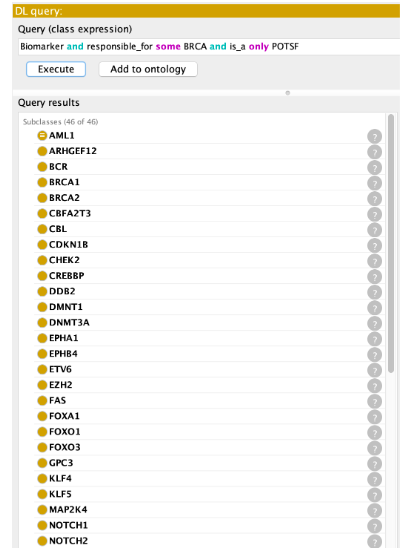
\includegraphics[width=0.45\linewidth,height=70mm]{images/sample_q_a.png}
	\caption{List of biomarkers classified as POTSF and responsible for breast cancer answered}
	\label{fig:sample_q_a}
	\vspace{-2mm}
\end{figure*}

\iffalse
\begin{figure}[th]
\vspace{-2mm}
\centering
\scriptsize
\begin{Verbatim}[frame=lines,numbers=left,numbersep=1pt]
SELECT ?otherEntity (count(?tweet) as ?count) WHERE {
  ?tweet schema:mentions ?entity ; dc:created ?date 
                FILTER(year(?date) = 2020 AND month(?date) = 4) .
  ?entity a nee:Entity ; nee:hasMatchedURI dbr:Donald_Trump .
  ?tweet schema:mentions ?entity2 . 
  ?entity2 a nee:Entity ; nee:hasMatchedURI ?otherEntity 
                FILTER (?otherEntity != dbr:Donald_Trump)
} GROUP BY ?otherEntity order by desc(?count) LIMIT 5
\end{Verbatim}
\vspace{-3mm}
\caption{Top entities co-occurring with the entity \textit{Donald Trump} during April 2020.}
\label{fig:sparqlEx1}
\vspace{-3mm}
\end{figure}
\fi 

\subsection{Interpretation of generated rules}
We interpret the inferred rules. We apply DLx Class Axiom Renderer Plugin\footnote{\url{https://github.com/MindfulMichaelJames/ProtegeDLAxiomPlugin}} to represent the rules.   

\subsubsection{Notations and assumptions}
Due to brevity, we cover some notations and assumptions that will be used for the interpretations:

\noindent i) if <Biomarker> $\sqsubseteq$ $\forall$is\_a.Protein-coding, following two rules implied:\\

\vspace{-6mm}
\begin{itemize}[noitemsep]
\scriptsize{
    \item Protein-coding$\sqsubseteq$ BiomarkerType
    \item BiomarkerType $\sqsubseteq$ Feature.}\\
\end{itemize}
\vspace{-6mm}

\noindent ii) if <Biomarker> $\sqsubseteq$ $\forall$is\_a.POTSF, following two rules implied:\\

\vspace{-6mm}
\begin{itemize}[noitemsep]
\scriptsize{
    \item POTSF$\sqsubseteq$ BiomarkerType
    \item BiomarkerType $\sqsubseteq$ Feature.} \\
\end{itemize}

\vspace{-6mm}
\noindent iii) if <Biomarker>$\sqsubseteq$ $\forall$is\_a.Oncogene, following two rules implied:\\

\vspace{-6mm}
\begin{itemize}[noitemsep]
\scriptsize{
    \item Oncogene $\sqsubseteq$ BiomarkerType
    \item BiomarkerType $\sqsubseteq$ Feature.} \\
\end{itemize}

\vspace{-6mm}
\noindent iv) for every disease ` responsible\_for<cancer-type>', the following three rules are implied:\\

\vspace{-6mm}
\begin{itemize}[noitemsep]
\scriptsize{
    \item <cancer-type>$\sqsubseteq$ Cancer
    \item Cancer$\sqsubseteq$DiseaseOfCellularProliferation
    \item DiseaseOfCellularProliferation$\sqsubseteq$Disease.}
\end{itemize}
\vspace{-2mm}

\subsubsection{Rules for subclasses}
We consider the following rules for features:

\vspace{-2mm}
\begin{itemize}[noitemsep]
\scriptsize{
    \item BiomarkerSignificance $ \sqsubseteq $ Feature
    \item BiomarkerType $ \sqsubseteq $ Feature
    \item Evidence $ \sqsubseteq $ Feature.}
\end{itemize}
\vspace{-2mm}

We consider the following rules on biomarker's significance:

\vspace{-2mm}
\begin{itemize}[noitemsep]
\scriptsize{
    \item High $ \sqsubseteq $  BiomarkerSignificance
    \item Low $ \sqsubseteq $  BiomarkerSignificance
    \item Medium $ \sqsubseteq $  BiomarkerSignificance
    \item Undefined $ \sqsubseteq $  BiomarkerSignificance.}
\end{itemize}
\vspace{-2mm}

\subsubsection{Rules associated with Biomarker Type}
We consider the following rules on biomarker types:

\vspace{-2mm}
\begin{itemize}[noitemsep]
\scriptsize{
    \item Oncogene $ \sqsubseteq $  BiomarkerType
    \item POTSF $ \sqsubseteq $  BiomarkerType
    \item Protein-coding $ \sqsubseteq $  BiomarkerType.}
\end{itemize}
\vspace{-2mm}

We consider the following rules on evidence types:

\vspace{-2mm}
\begin{itemize}[noitemsep]
\scriptsize{
    \item CancerIndex $ \sqsubseteq $  Evidence
    \item MeSH $ \sqsubseteq $  Evidence
    \item PubMed $ \sqsubseteq $  Evidence}
\end{itemize}
\vspace{-2mm}

\subsubsection{Rules by cancer types}
As already mention, we consider the following cancer types:

\vspace{-2mm}
\begin{itemize}[noitemsep]
\scriptsize{
  \item DiseaseOfCellularProliferation  $\sqsubseteq $ Disease
  \item Cancer $\sqsubseteq $ DiseaseOfCellularProliferation
  \item AcuteLymphocyticLeukaemia $ \sqsubseteq $ Cancer
  \item UrinaryBladderCancer $ \sqsubseteq $ Cancer
  \item BreastCancer $ \sqsubseteq $ Cancer
  \item Carcinoid $ \sqsubseteq $ Cancer
    \item ChronicLymphocyticLeukemia $ \sqsubseteq $ Cancer
  \item ColorectalCancer $ \sqsubseteq $ Cancer
  \item DiffuseLargeB-cellLymphoma $ \sqsubseteq $ Cancer
  \item EsophagealCancer $ \sqsubseteq $ Cancer
  \item GlioblastomaMultiforme $ \sqsubseteq $ Cancer
  \item HeadAndNeckCancer $ \sqsubseteq $ Cancer
 \item KidneyClearCell $ \sqsubseteq $ Cancer
  \item AcuteMyleoidLeukemia $ \sqsubseteq $ Cancer
    \item LungAdenocarcinoma $ \sqsubseteq $ Cancer
  \item LungSquasmousCellCarcinoma $ \sqsubseteq $ Cancer
  \item Medulloblastoma $ \sqsubseteq $ Cancer
  \item Melanoma $ \sqsubseteq $ Cancer
  \item MultipleMyeloma $ \sqsubseteq $ Cancer
  \item Neuroblastoma $ \sqsubseteq $ Cancer
  \item OvarianCancer $ \sqsubseteq $ Cancer
    \item PanCan $ \sqsubseteq $ Cancer
      \item ProstateCancer $ \sqsubseteq $ Cancer
  \item EndometrialCancer $ \sqsubseteq $ Cancer
  \item RhabdoidCancer $ \sqsubseteq $ Cancer.}
\end{itemize}
\vspace{-4mm}

\subsubsection{Rules by biomarkers}
For all the biomarkers, we have generated as much as 1,900 rules. However, for the brevity, we represent the following rule set for a few representative biomarkers only. First, we provide the rule set for biomarker, `AKT1'. The serine-threonine protein kinase encoded by the AKT1 gene is catalytically inactive in serum-starved primary and immortalized fibroblasts. AKT1 and the related AKT2 are activated by platelet-derived growth factor. The activation is rapid and specific, and it is abrogated by mutations in the pleckstrin homology domain of AKT1. It was shown that the activation occurs through phosphatidylinositol 3-kinase. In the developing nervous system AKT1 is a critical mediator of growth factor-induced neuronal survival. Survival factors can suppress apoptosis in a transcription-independent manner by activating the serine or threonine kinase AKT1, which then phosphorylates and inactivates components of the apoptotic machinery. Mutations in this gene have been associated with the Proteus syndrome. Multiple alternatively spliced transcript variants have been found for this gene: 

%\vspace{-2mm}
\begin{itemize}[noitemsep]
\scriptsize{
    \item AKT1 $ \sqsubseteq  $ Biomarker
    \item AKT1 $ \sqsubseteq  $ $\exists$is$ {\_}$a.Oncogene
    \item AKT1 $ \sqsubseteq  $ ($\exists$has$ {\_}$significance$ {\_}$degree.High) $  \cap $ ($\exists$responsible$ {\_}$for.PanCan)
    \item AKT1 $ \sqsubseteq  $ ($\exists$has$ {\_}$evidence.PubMed) $  \cap $ ($\exists$has$ {\_}$significance$ {\_}$degree.Low) $  \cap $ ($\exists$responsible$ {\_}$for.UrinaryBladderCancer)
    \item AKT1 $ \sqsubseteq  $ ($\exists$has$ {\_}$significance$ {\_}$degree.Medium) $  \cap $ ($\exists$responsible$ {\_}$for.EndometrialCancer).}
\end{itemize}
%\vspace{-2mm}

\hspace*{3.5mm} Preceding rule set signifies that AKT1 is an oncogene biomarker responsible for both PanCan, urinary bladder, and endmetrical cancer types, with significance being high, low, and medium, respectively. To show more detail coverage, we provide rule set for another biomarker called `TP53', which encodes a tumor suppressor protein containing transcriptional activation\footnote{\url{https://www.ncbi.nlm.nih.gov/gene/7157}}, DNA binding, and oligomerization domains. The encoded protein responds to diverse cellular stresses to regulate expression of target genes, thereby inducing cell cycle arrest, apoptosis, senescence, DNA repair, or changes in metabolism. Mutations in this gene are associated with a variety of human cancers, including hereditary cancers such as Li-Fraumeni syndrome. Alternative splicing of this gene and the use of alternate promoters result in multiple transcript variants and isoforms. Additional isoforms result from the use of alternate translation initiation codons. 

\begin{itemize}[noitemsep]
\scriptsize{
    \item TP53 $ \sqsubseteq  $ Biomarker
    \item TP53 $ \sqsubseteq  $ $  \forall $is$ {\_}$a.Protein-coding
    \item TP53 $ \sqsubseteq  $ $  \forall $is$ {\_}$a.POTSF
    \item TP53 $ \sqsubseteq  $ ($\exists$has$ {\_}$evidence.PubMed) $  \cap $ ($\exists$has$ {\_}$significance$ {\_}$degree.High) $  \cap $ ($\exists$responsible$ {\_}$for.EndometrialCancer)
    \item TP53 $ \sqsubseteq  $ ($\exists$has$ {\_}$significance$ {\_}$degree.High) $  \cap $ ($\exists$responsible$ {\_}$for.LungSquasmousCellCarcinoma)
    \item TP53 $ \sqsubseteq  $ ($\exists$has$ {\_}$significance$ {\_}$degree.High) $  \cap $ ($\exists$responsible$ {\_}$for.GlioblastomaMultiforme)
    \item TP53 $ \sqsubseteq  $ ($\exists$has$ {\_}$significance$ {\_}$degree.High) $  \cap $ ($\exists$responsible$ {\_}$for.PanCan)
    \item TP53 $ \sqsubseteq  $ ($\exists$has$ {\_}$significance$ {\_}$degree.High) $  \cap $ ($\exists$responsible$ {\_}$for.LungAdenocarcinoma)
    \item TP53 $ \sqsubseteq  $ ($\exists$has$ {\_}$significance$ {\_}$degree.High) $  \cap $ ($\exists$responsible$ {\_}$for.KidneyClearCell)
    \item TP53 $ \sqsubseteq  $ ($\exists$has$ {\_}$evidence.PubMed) $  \cap $ ($\exists$has$ {\_}$significance$ {\_}$degree.High) $  \cap $ ($\exists$responsible$ {\_}$for.UrinaryBladderCancer)
    \item TP53 $ \sqsubseteq  $ ($\exists$has$ {\_}$evidence.PubMed) $  \cap $ ($\exists$has$ {\_}$significance$ {\_}$degree.High) $  \cap $ ($\exists$responsible$ {\_}$for.ColorectalCancer)
    \item TP53 $ \sqsubseteq  $ ($\exists$has$ {\_}$evidence.PubMed) $  \cap $ ($\exists$has$ {\_}$significance$ {\_}$degree.High) $  \cap $ ($\exists$responsible$ {\_}$for.EsophagealCancer)
    \item TP53 $ \sqsubseteq  $ ($\exists$has$ {\_}$significance$ {\_}$degree.High) $  \cap $ ($\exists$responsible$ {\_}$for.DiffuseLargeB-cellLymphoma)
    \item TP53 $ \sqsubseteq  $ ($\exists$has$ {\_}$evidence.PubMed) $  \cap $ ($\exists$has$ {\_}$significance$ {\_}$degree.Low) $  \cap $ ($\exists$responsible$ {\_}$for.Medulloblastoma)
    \item TP53 $ \sqsubseteq  $ ($\exists$has$ {\_}$evidence.PubMed) $  \cap $ ($\exists$has$ {\_}$significance$ {\_}$degree.High) $  \cap $ ($\exists$responsible$ {\_}$for.OvarianCancer)
    \item TP53 $ \sqsubseteq  $ ($\exists$has$ {\_}$evidence.PubMed) $  \cap $ ($\exists$has$ {\_}$significance$ {\_}$degree.High) $  \cap $ ($\exists$responsible$ {\_}$for.ChronicLymphocyticLeukemia)
   % \item TP53 $ \sqsubseteq  $ ($\exists$has$ {\_}$evidence.PubMed) $  \cap $ ($\exists$has$ {\_}$significance$ {\_}$degree.High) $  \cap $ ($\exists$responsible$ {\_}$for.BreastCancer)
    \item TP53 $  \cap $ ($\exists$has$ {\_}$significance$ {\_}$degree.High) $  \cap $ ($\exists$responsible$ {\_}$for.BreastCancer) $ \sqsubseteq  $ ($\exists$has$ {\_}$evidence.PubMed) $\cap$ (=493) (has ${\_}$citations.T)
    \item TP53 $ \sqsubseteq  $ ($\exists$has$ {\_}$significance$ {\_}$degree.High) $  \cap $ ($\exists$responsible$ {\_}$for.MultipleMyeloma)
    \item TP53 $ \sqsubseteq  $ ($\exists$has$ {\_}$evidence.PubMed) $  \cap $ ($\exists$has$ {\_}$significance$ {\_}$degree.Medium) $  \cap $ ($\exists$responsible$ {\_}$for.ProstateCancer)
    \item TP53 $ \sqsubseteq  $ ($\exists$has$ {\_}$evidence.PubMed) $  \cap $ ($\exists$has$ {\_}$significance$ {\_}$degree.High) $  \cap $ ($\exists$responsible$ {\_}$for.Melanoma)
    \item TP53 $ \sqsubseteq  $ ($\exists$has$ {\_}$significance$ {\_}$degree.Low) $  \cap $ ($\exists$responsible$ {\_}$for.Carcinoid)
    \item TP53 $ \sqsubseteq  $ ($\exists$has$ {\_}$significance$ {\_}$degree.High) $  \cap $ ($\exists$responsible$ {\_}$for.HeadAndNeckCancer.)}
\end{itemize}

\subsection{Decision reasoning with rules}
The preceding rule set covers a couple of facts w.r.t. the cancer types such as significance, mutations associations with cancer types, PubMed association, and conforming gene types. We now analyse the above rules by breaking down into smaller assertions: 
\vspace{-2mm}

\begin{itemize}[noitemsep]
\scriptsize{
    \item TP53 is a biomarker
    \item TP53 is a protein-coding gene
    \item TP3 is has both oncogenic and tumor-suppressor functions, i.e., they have both oncogenic and tumor-suppressor functionality. 
    \item TP53 is responsible for 19 different cancers which is supported in TumorPortal\footnote{\url{http://www.tumorportal.org/view?geneSymbol=TP53}}
    \item TP53 has high significance w.r.t. different cancer types, given it is very reactive to changes to mutations \& gene expression. 
    \item TP53 is well studied biomarkers with strong scientific publication support, i.e., PubMed association. For example, for the breast cancer as many as 493 papers have confirmed TP53,s association with it.  
    \item For some cancer types, TP53 has low significance, for which however we can't confidently say that we can discard their association w.r.t for that cancer types. 
    \item Although TP53 is not an oncogene, it's evidently found  responsible for different cancer types. }
\end{itemize}

\hspace*{3.5mm} Now relating this rule set with the decision rules can be described with an example. Suppose, a doctor uploads patient's multimodal genomic data~(or unimodal in restrictive scenario) to get the diagnosis decision. Based on the outcome at hand~(e.g., prediction, feature importance, decision rule set), he then can be ensured that the patient has breast cancer. Subsequently, he can explain that the model made such decision by exposing blood biomarkers role, e.g., TP53 is the most significant biomarkers. Further, upon the patient request, doctor can then write a SPARQL or DLx query and ask the reasoner to reason how the decision is deduced/inferred based on the following rules and domain-knowledge he is aware of:  

\begin{itemize}[noitemsep]
\scriptsize{
    \item TP53 $ \sqsubseteq  $ Biomarker
    \item TP53 $ \sqsubseteq  $ $  \forall $is$ {\_}$a.Protein-coding
    \item TP53 $ \sqsubseteq  $ $  \forall $is$ {\_}$a.POTSF
    \item TP53 $  \cap $ ($\exists$has$ {\_}$significance$ {\_}$degree.High) $  \cap $ ($\exists$responsible$ {\_}$for.BreastCancer) $ \sqsubseteq  $ ($\exists$has$ {\_}$evidence.PubMed) $\cap$ (=493) (has ${\_}$citations.T)}
\end{itemize}

\hspace*{3.5mm} Additinally, the doctor can interpret this rule to the patient, where the decision is backed by the fact that a gene biomarker called `TP53': `TP53' is found to be highly responsible for the presence of breast cancer in your body. This gene has very strong mutations associations w.r.t. to breast cancer. Nevertheless, many scientific article has found it's association. What we assume that such an inferred rule can be used not only to fix inconsistencies, but also to generate fairer decision rules. 

\section{Chapter Summary}\label{chapter_8:conclusion}
In this chapter, the semantic layer that we developed consists of the query processing module, instance classifier, and ontological reasoner~\cite{futia2020integration}. Our approach based on SW technologies offer a data-efficient process by which models can be trained to reason on symbolic contexts and are able to provide background knowledge for DL models. We developed a domain-specific ontology as the basis of the KB by reusing concepts and knowledge from existing ontologies and KBs. We show how the SR can infer domain knowledge about top-k biomarkers we already identified. 
Besides, we validate diagnoses decision based on domain knowledge from the KB. 
Generated rules are not only statistically evident, but also validated based on the domain-knowledge from several external sources that we embedded in our KG. 

\hspace*{3.5mm} However, several potential limitations of our approach leaves many improvement possibilities. First, considering their features, symbolic methods are not robust to noise and can not be applied to non-symbolic context, where the data is ambiguous~\cite{futia2020integration}. Second, the expressiveness of DLx is not tested against incompleteness and inconsistency. In the same line, formalizing the queries in SPARQL syntax and querying the ontology against SPARQL endpoint could be an option. Third, the list of NLQ and DLQ shown in \cref{table:nlq_dlq} is not comprehensive as well hard-coded. The outlook is formulating more such rules and use them in question answering over the KG. Fourth, we could use the fully inferred, deductively closed knowledge graph to perform  embeddings. Such KG embeddings on the deductively closed graph would have  the advantage that not only asserted axioms will be taken into consideration, but representations can also include inferred knowledge that is not present explicitly in the graph~\cite{alshahrani2017neuro}. 

\hspace*{3.5mm}Since KG embeddings can be applied in numerous task ranging from link prediction to recommendation systems. The advantage would be that the generated embeddings would contain both explicit and implicit information through the use of symbolic logic, which gives opportunities of link predictions tasks including, finding candidate genes of diseases, protein-protein interactions, and drug target predictions. Since an efficient ML model maybe better at predicting, detecting, and processing patterns then a human being, it may provide bias decision. Therefore, it is important to take fairness issues into consideration while developing such an XAI system, because such systems can be used in many sensitive environments to make important and life-changing decisions~\cite{stiglic2020interpretability}. Besides, it is essential to ensure that the decisions do not reflect discriminatory behavior toward certain groups or populations~\cite{mehrabi2019survey}. 

\hspace*{3.5mm} Through several post-hoc interpretability and explainability methods, we have seen uncovering algorithmic discrimination was relatively easier than developing fair clinical diagnostics decision support system~(CDSS) because we generated explanations based on mathematical and statistical exercises. Although, decision made by the model has to be explainable and fair, which is not possible to say how interpretable and fair our approach without assessing them. Considering these requirements and motivations, we will assess both from statistical and philosophical perspective in the next chapter. Nevertheless, we show how to generate fair decision rules by combing the inferred rules and the rule set we generated in \cref{chapter:xai_rules}, i.e., we combine rules based on statistical rules and inferred rules and modify.% if necessary. 

	\vspace{-2mm}

